\documentclass[../thesis.tex]{subfiles}

\begin{document}

\chapter{Real World Testing}

\section{Aim}

Verifying the the proposed system is working well with real devices on a small scale.

\section{Setup} % Things to do before the experiment.

The solar power generation setup is documented in the figure \ref{fig:realworldsensing}. In summary, the solar panel generates electricity, which is measured by the input sensor and fed into the converter. After converting to the desired voltage, the electricity is measured by the output sensor and stored in the battery. Additionally, there is an inverter that converts the DC electricity from the battery to AC. The electricity is then used to power the load and the microcontroller where the load in the experimental setup is a portable air conditioning unit. Finally, the power generation and charging circuit, and the power inverter circuit are proctected by the circuit breakers. The real world setup is shown in the figure \ref{fig:realworld1}, \ref{fig:realworld2}, and \ref{fig:realworld3}. It is functionally equivalent to the setup in figure \ref{fig:realworldsensing}.

\begin{figure}[!ht]
	\centering
	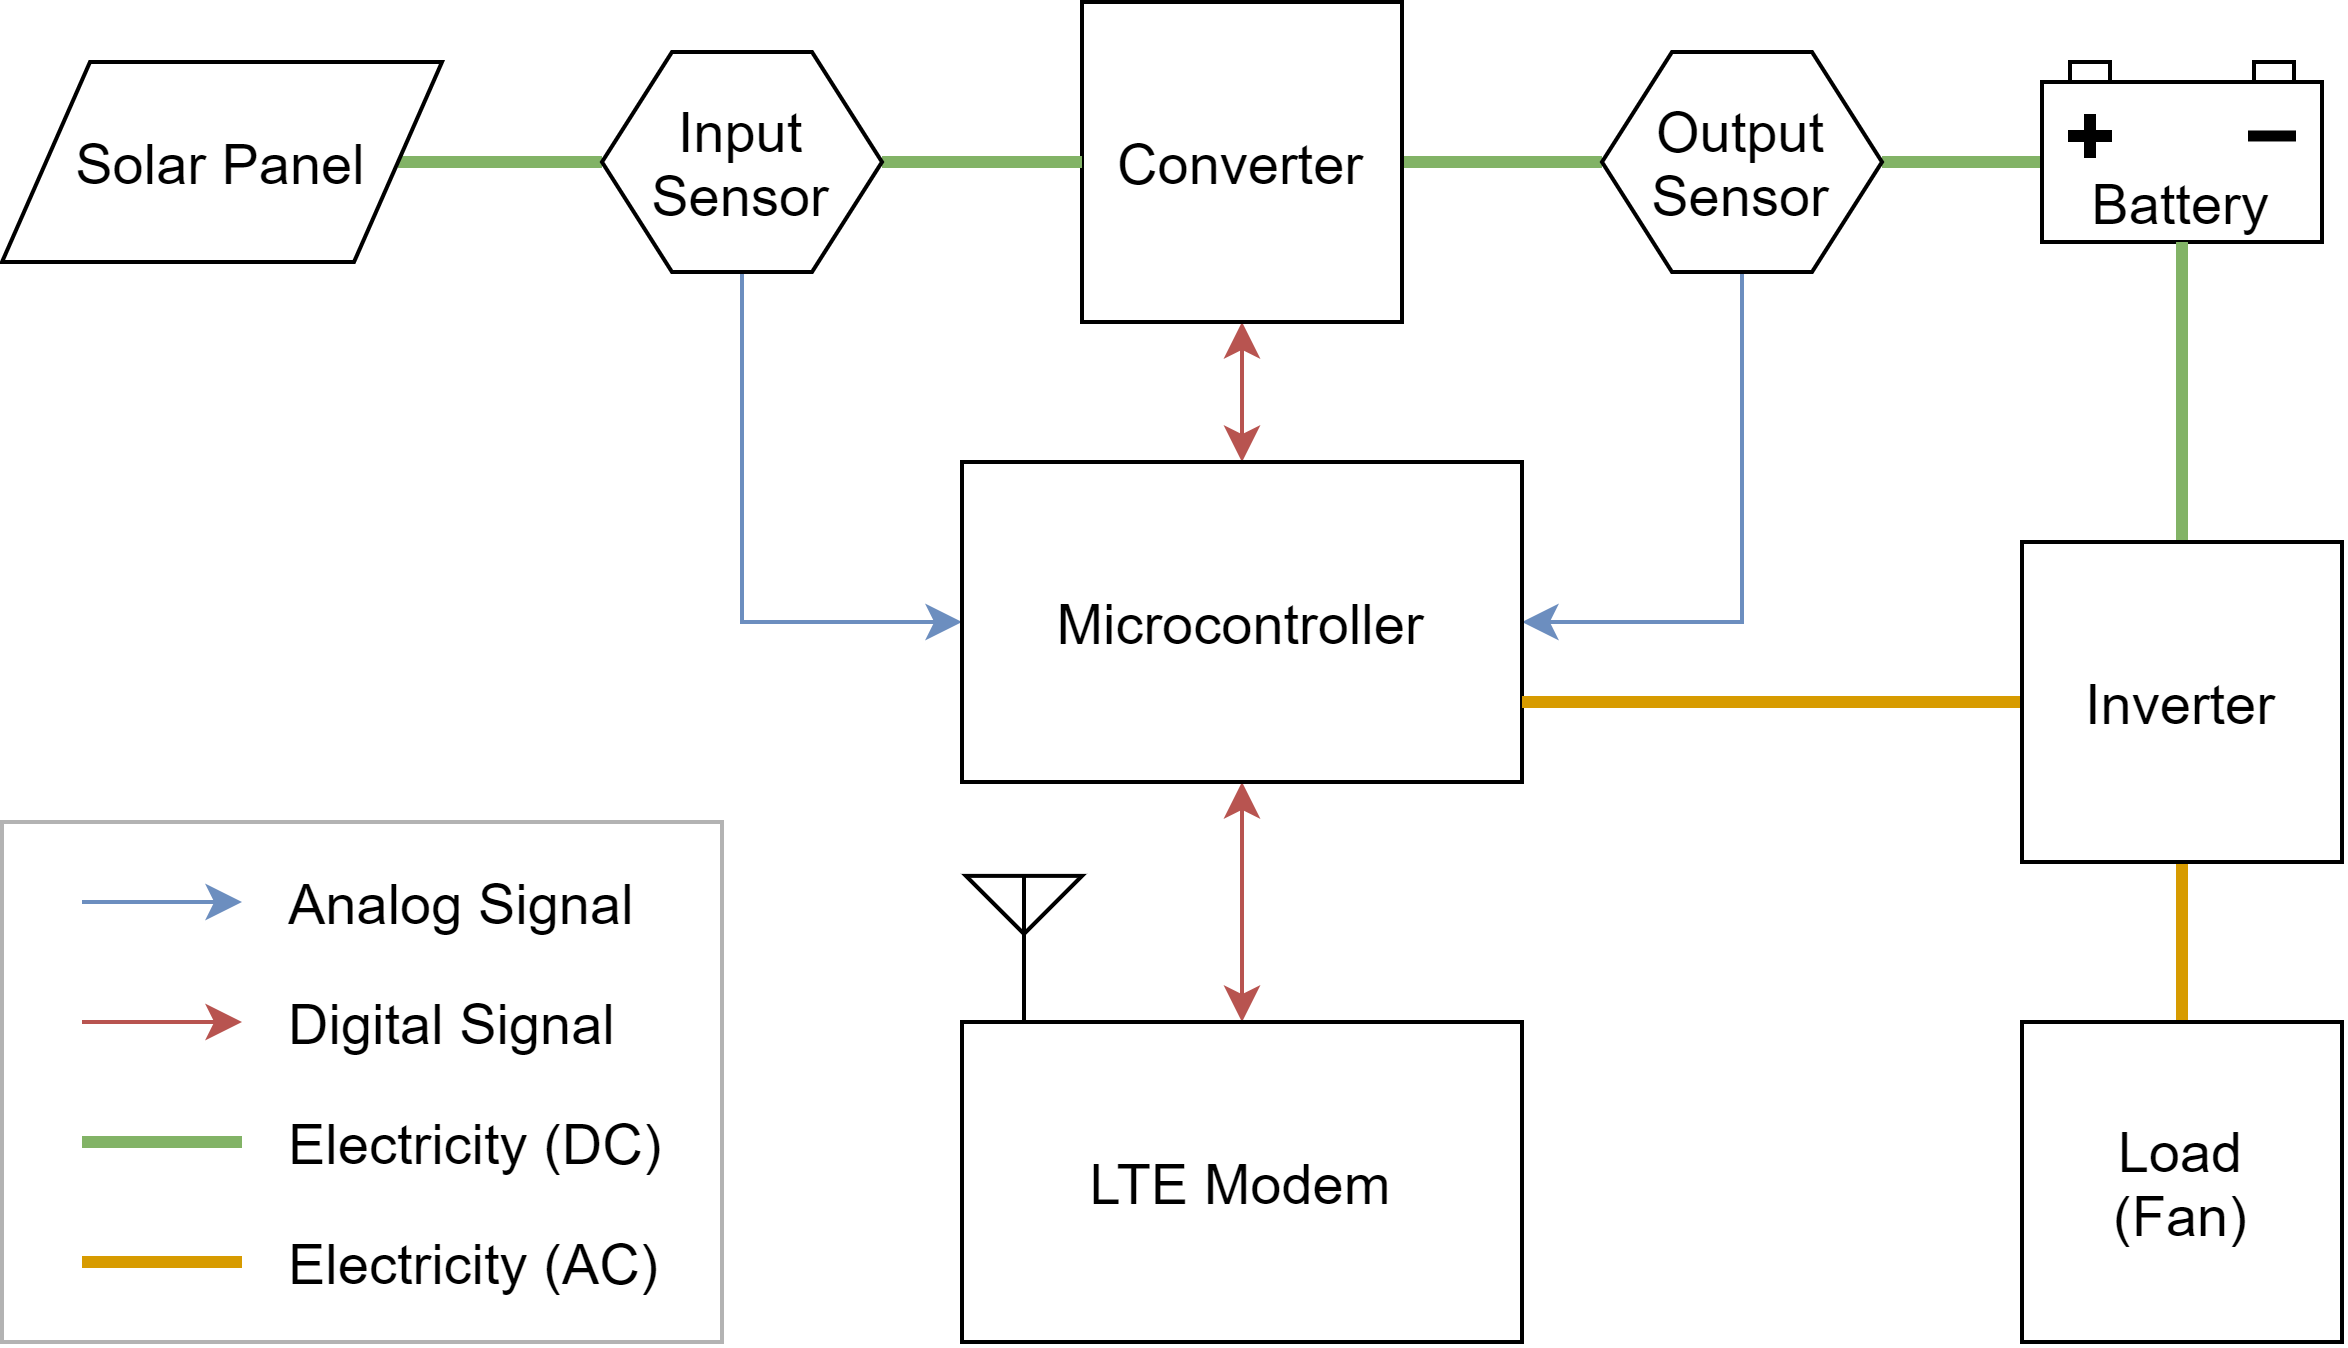
\includegraphics[width=\linewidth]{c6-sensing.png}
	\caption{The experimental setup (Schematic)}
	\label{fig:realworldsensing}
\end{figure}

The proposed system is deployed to an Elastic Compute Cloud (Amazon EC2) instance of type T2.Micro and the components are running inside Docker Containers. Finally, the firewall is configured to allow public access to the frontend and backend servers. 

A sim card with a 4G data plan is inserted into the microcontroller and the modem is connected to the microcontroller through the mini-PCIe slot. The antenna must be attached to the MAIN connector of the modem to communicate with any LTE base station. Additionally, the external power cable supplies power to the LTE modem, and the board power cable supplies power to the microcontroller, both cables must be connected to the board for the controller and modem to work properly together. The setup is shown in the figure \ref{fig:realworld4}. 

Configurations of the sim card is either set ahead of firmware compile time or detected automatically from the mobile service provider.

\begin{figure}[!ht]
	\centering
	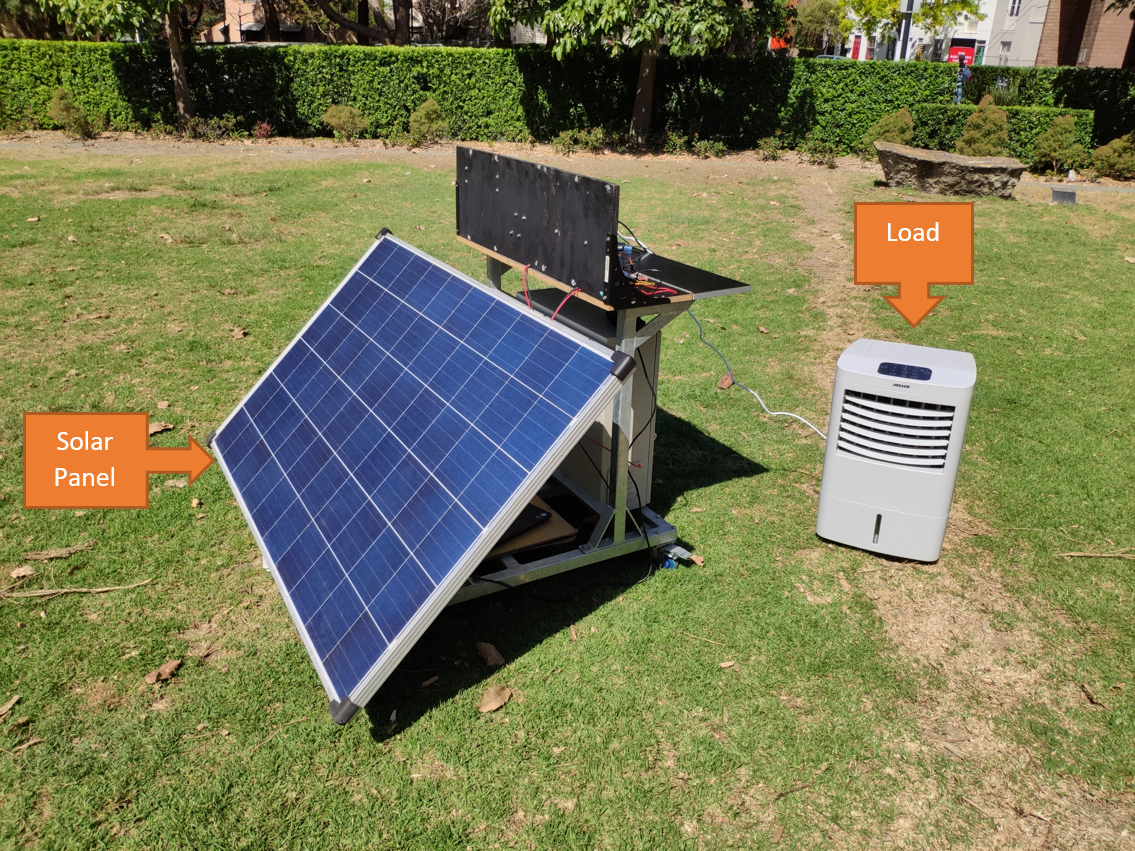
\includegraphics[width=0.8\linewidth]{realworld1.png}
	\caption{The experimental setup (front)}
	\label{fig:realworld1}
\end{figure}

\begin{figure}[!ht]
	\centering
	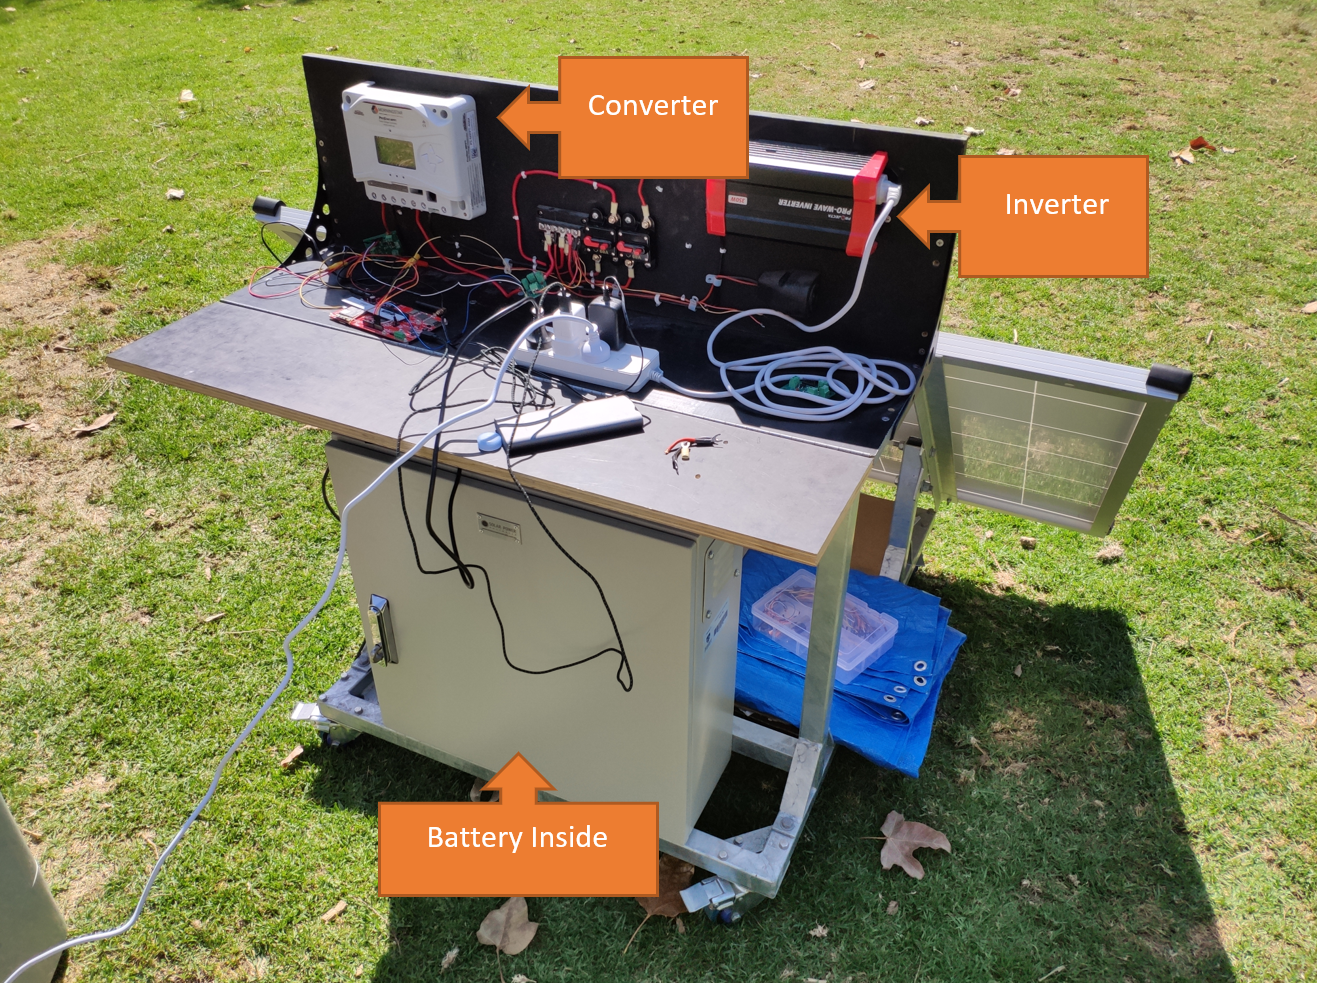
\includegraphics[width=0.8\linewidth]{realworld2.png}
	\caption{The experimental setup (back)}
	\label{fig:realworld2}
\end{figure}

\begin{figure}[!ht]
	\centering
	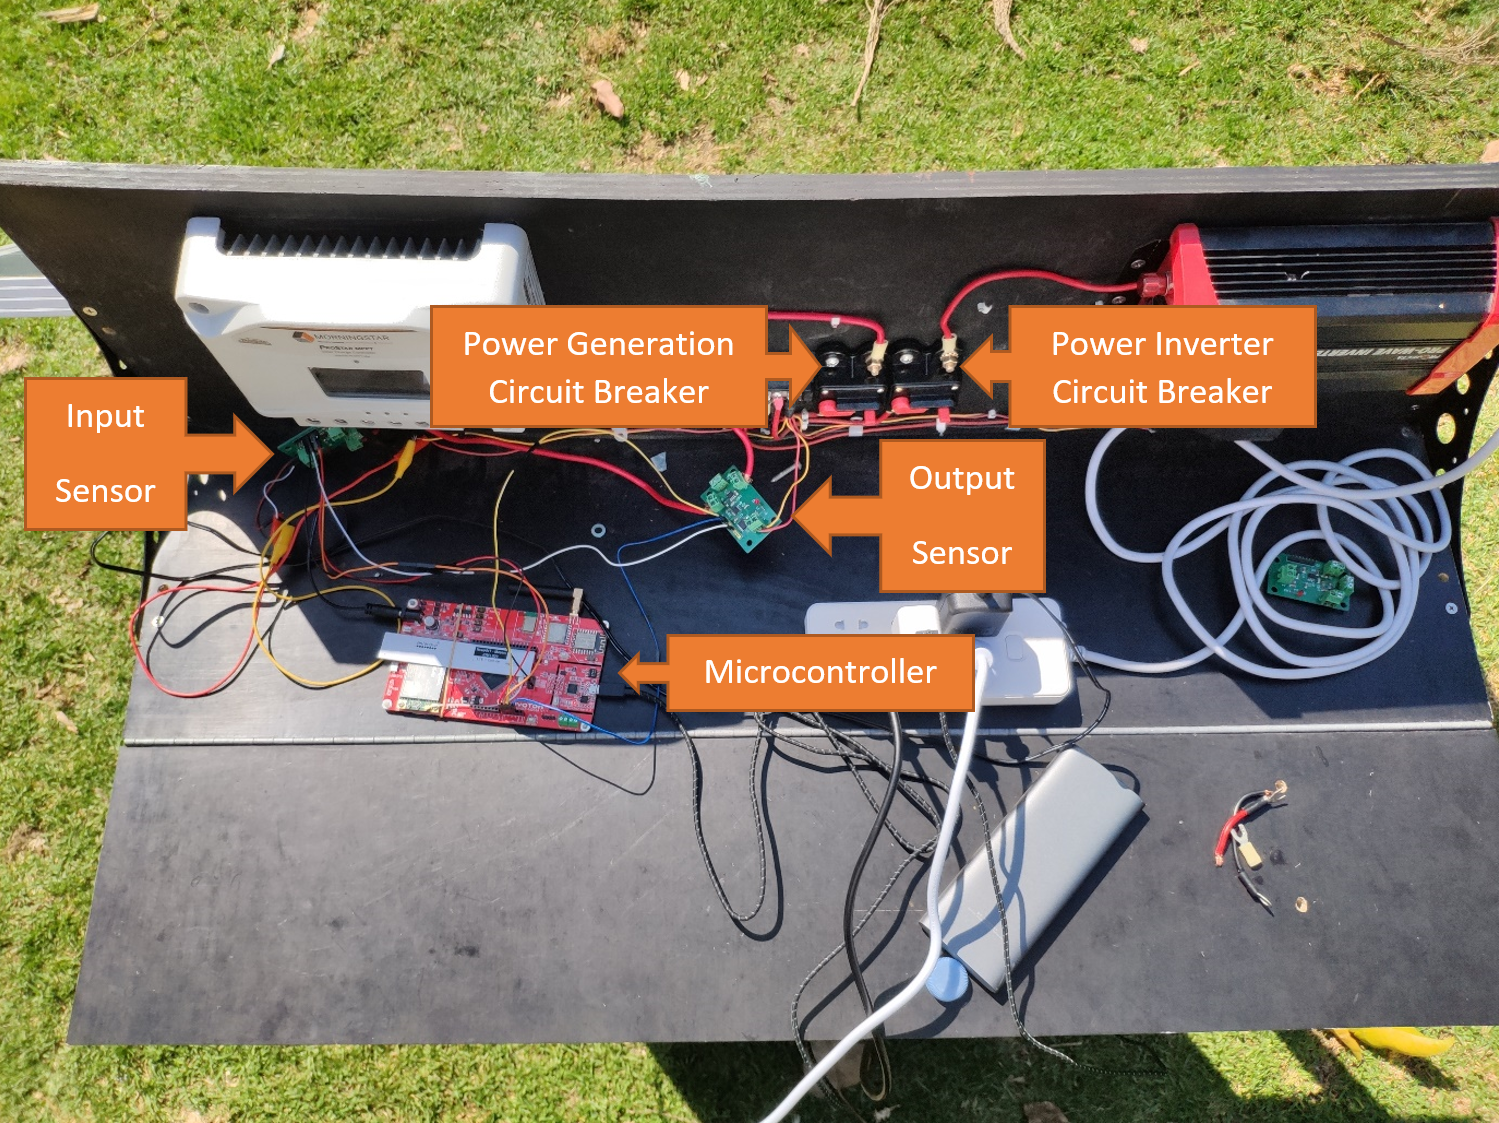
\includegraphics[width=0.8\linewidth]{realworld3.png}
	\caption{The experimental setup (top)}
	\label{fig:realworld3}
\end{figure}

\begin{figure}[!ht]
	\centering
	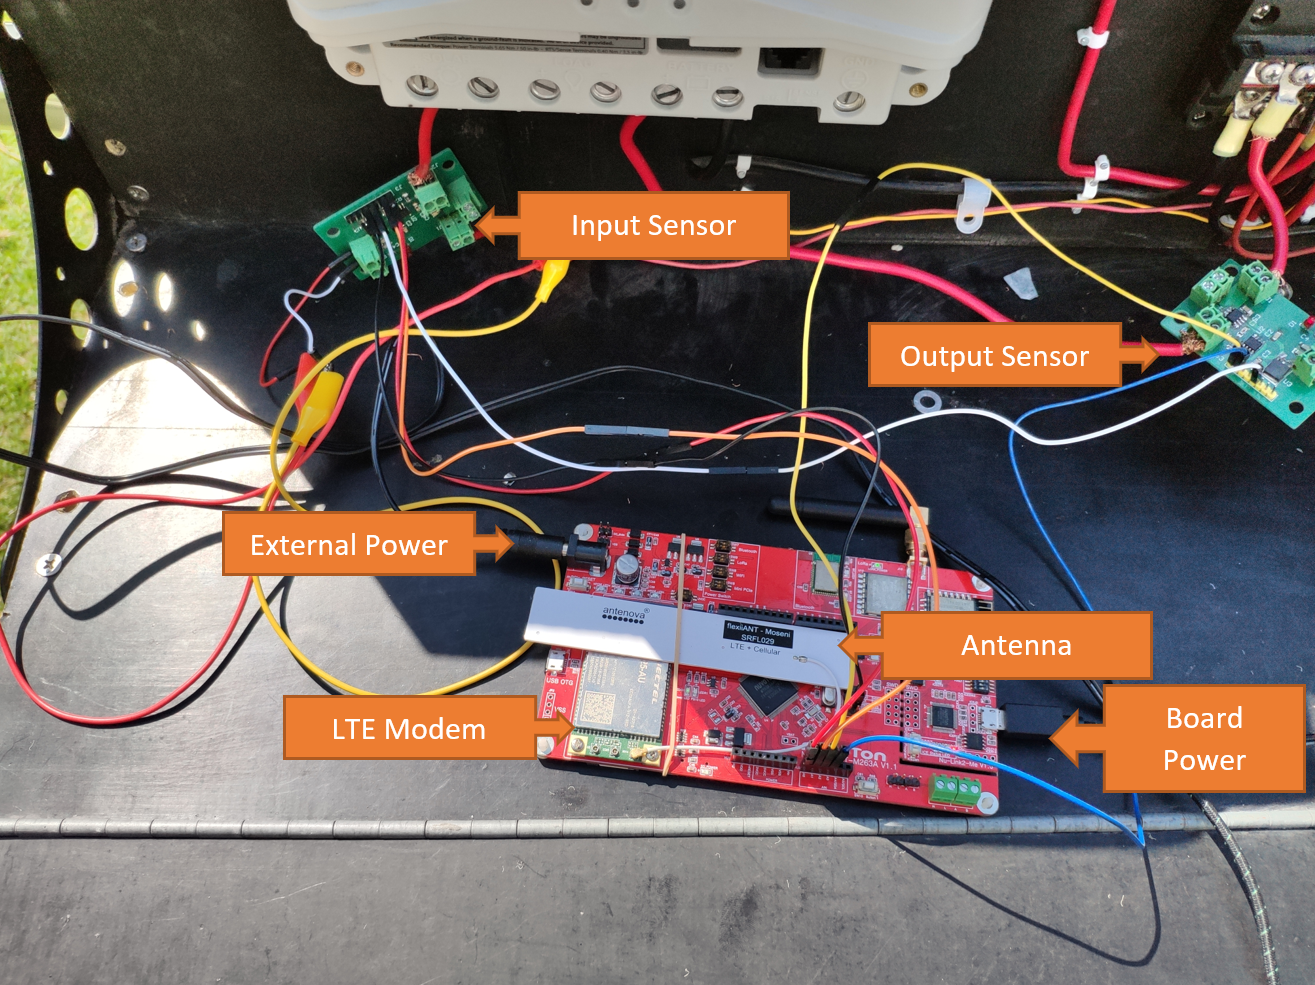
\includegraphics[width=0.8\linewidth]{realworld4.png}
	\caption{The experimental setup (controller)}
	\label{fig:realworld4}
\end{figure}

\section{Procedures} % Things to do during the experiment

The starting phase follows the following procedures:

\begin{itemize}
	\item Inspect the experimental setup is connected properly.
	\item Turn on the circuit breaker to enable the power generation and charging circuit. 
	\item Turn on the cirtuit breaker to enable the power inverter circuit. 
	\item Connect the microcontroller to the external power.
	\item Connect the microcontroller to the board power.
	\item Access the website and verify the data are being recorded.
\end{itemize}

After recording data for at least two hours, the setup can be safely shutdown by using the following procedures:

\begin{itemize}
	\item Shutdown the device from the website.
	\item Disconnect the microcontroller from the external power.
	\item Disconnect the microcontroller from the board power.
	\item Turn off the circuit breaker to disable the power inverter circuit.
	\item Turn off the circuit breaker to disable the power generation and charging circuit.
	\item Inspect any damages caused by the experiments.
\end{itemize}

A failure scenario is simulated by disconnecting the microcontroller power directly instead of shutting it down from the website first, this can be used to verify the system is able to detect a device is terminated unexpectedly. 

\section{Analysis}

The weather on day of testing was sunny and cloudless, the testing is performed from 1:30PM to 3:30PM on a typical Sydney summary day. After a recording for a period of two hours, there are three types of data that are recorded on the system.

\begin{itemize}
	\item Device Information
	\item Aggregate Statistics
	\item Realtime Statistics
\end{itemize}

As shown in the figure \ref{fig:page1}, the device information section shows the experimental setup is assigned a globally unique device ID \em IOfaSZKA \em for identification. The region is currently within the \em Awaiting Allocation \em region, which is a region to accomodate devices with no specific region assignment. The operating status of the device is \em Online \em, the status would be \em Offline \em if the device terminates properly. Otherwise, the \em Failure \em status will be shown in the status, indicating the device has not terminate properly. The listening port is the ID of the server that it is getting data from. 

\begin{figure}[!ht]
	\centering
	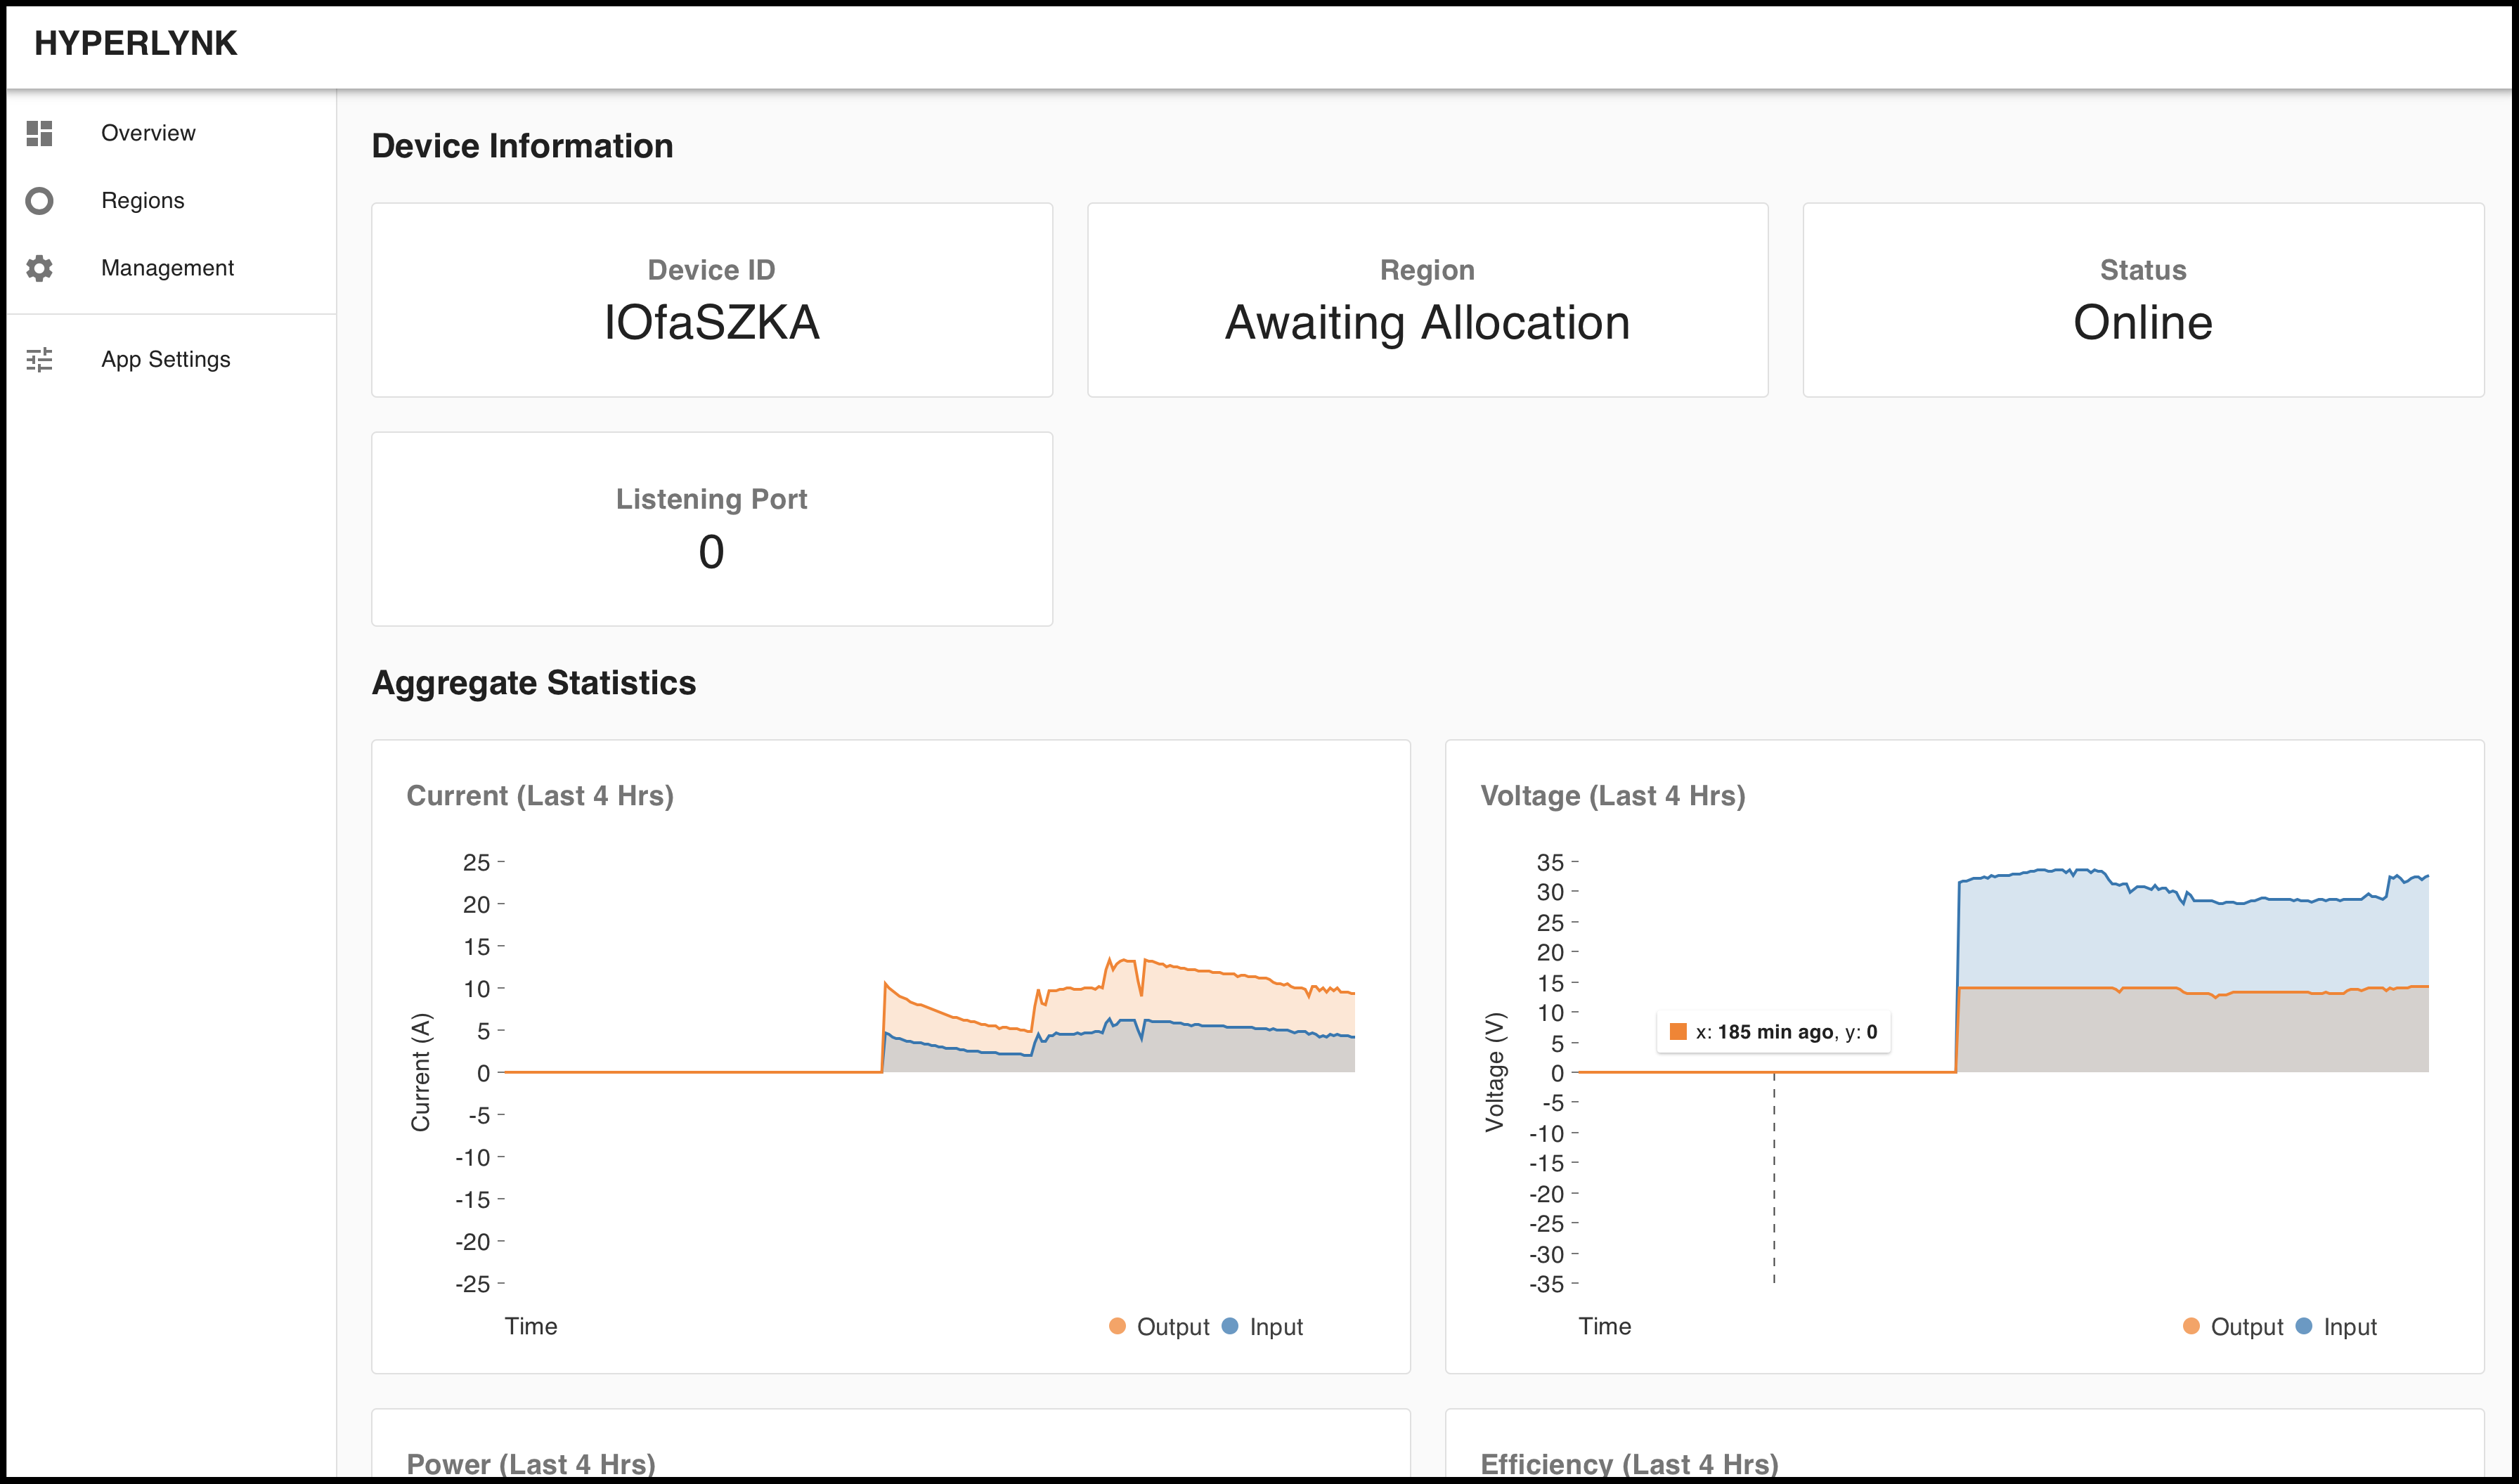
\includegraphics[width=\linewidth]{page1.png}
	\caption{The website showing the device information.}
	\label{fig:page1}
\end{figure}

In the figure \ref{fig:page2}, the aggregate statistics section shows the recorded data over a period of 4 hours and each data point represents the average value for that minute. For clarity, the recorded aggregate data is redrawn in the figure \ref{fig:captured}. Since the focus of this thesis is on the communication system and doesn't include the data measuring, which is done by another research student. I would only provide a brief discussion regarding the data here. From the beginning of the test to the 40 minutes mark, the converter is charging the battery and the battery is about to reach its maximum capacity, which is the reason of the current is slowing decreasing and voltage is slowly increasing over time. The increase in power from 40 to 60 minutes mark is caused by a laptop that is charging through the inverter and the converter adjust the power to compensate for the load. The further increase in power from 60 minutes mark is when a portable air conditioning unit is powered on. Again, the increase in power is due to the converter is compensating for the additional load. It is also worth mentioning that the power is slowly decreasing after the 60 minutes mark, the reason for the decrease in power is the portable air conditioning unit rely on water to keep things cool and the water is slowly running out over the course of the testing, resulting in decrease in power draw. The negative spikes in the recorded data is when the experiment setup is being modified such as introducing or removing loads. Interestingly, the efficiency during the test exceeded 100\% very occasionally, which is not physically possible. We later found out the sensors were not calibrated properly and the data reported to the proposed system contains the measuring error. Since this is not the focus of the thesis, the experiment is still considered success as it had demonstrated the critical functionalities are working. 

\begin{figure}[!ht]
	\centering
	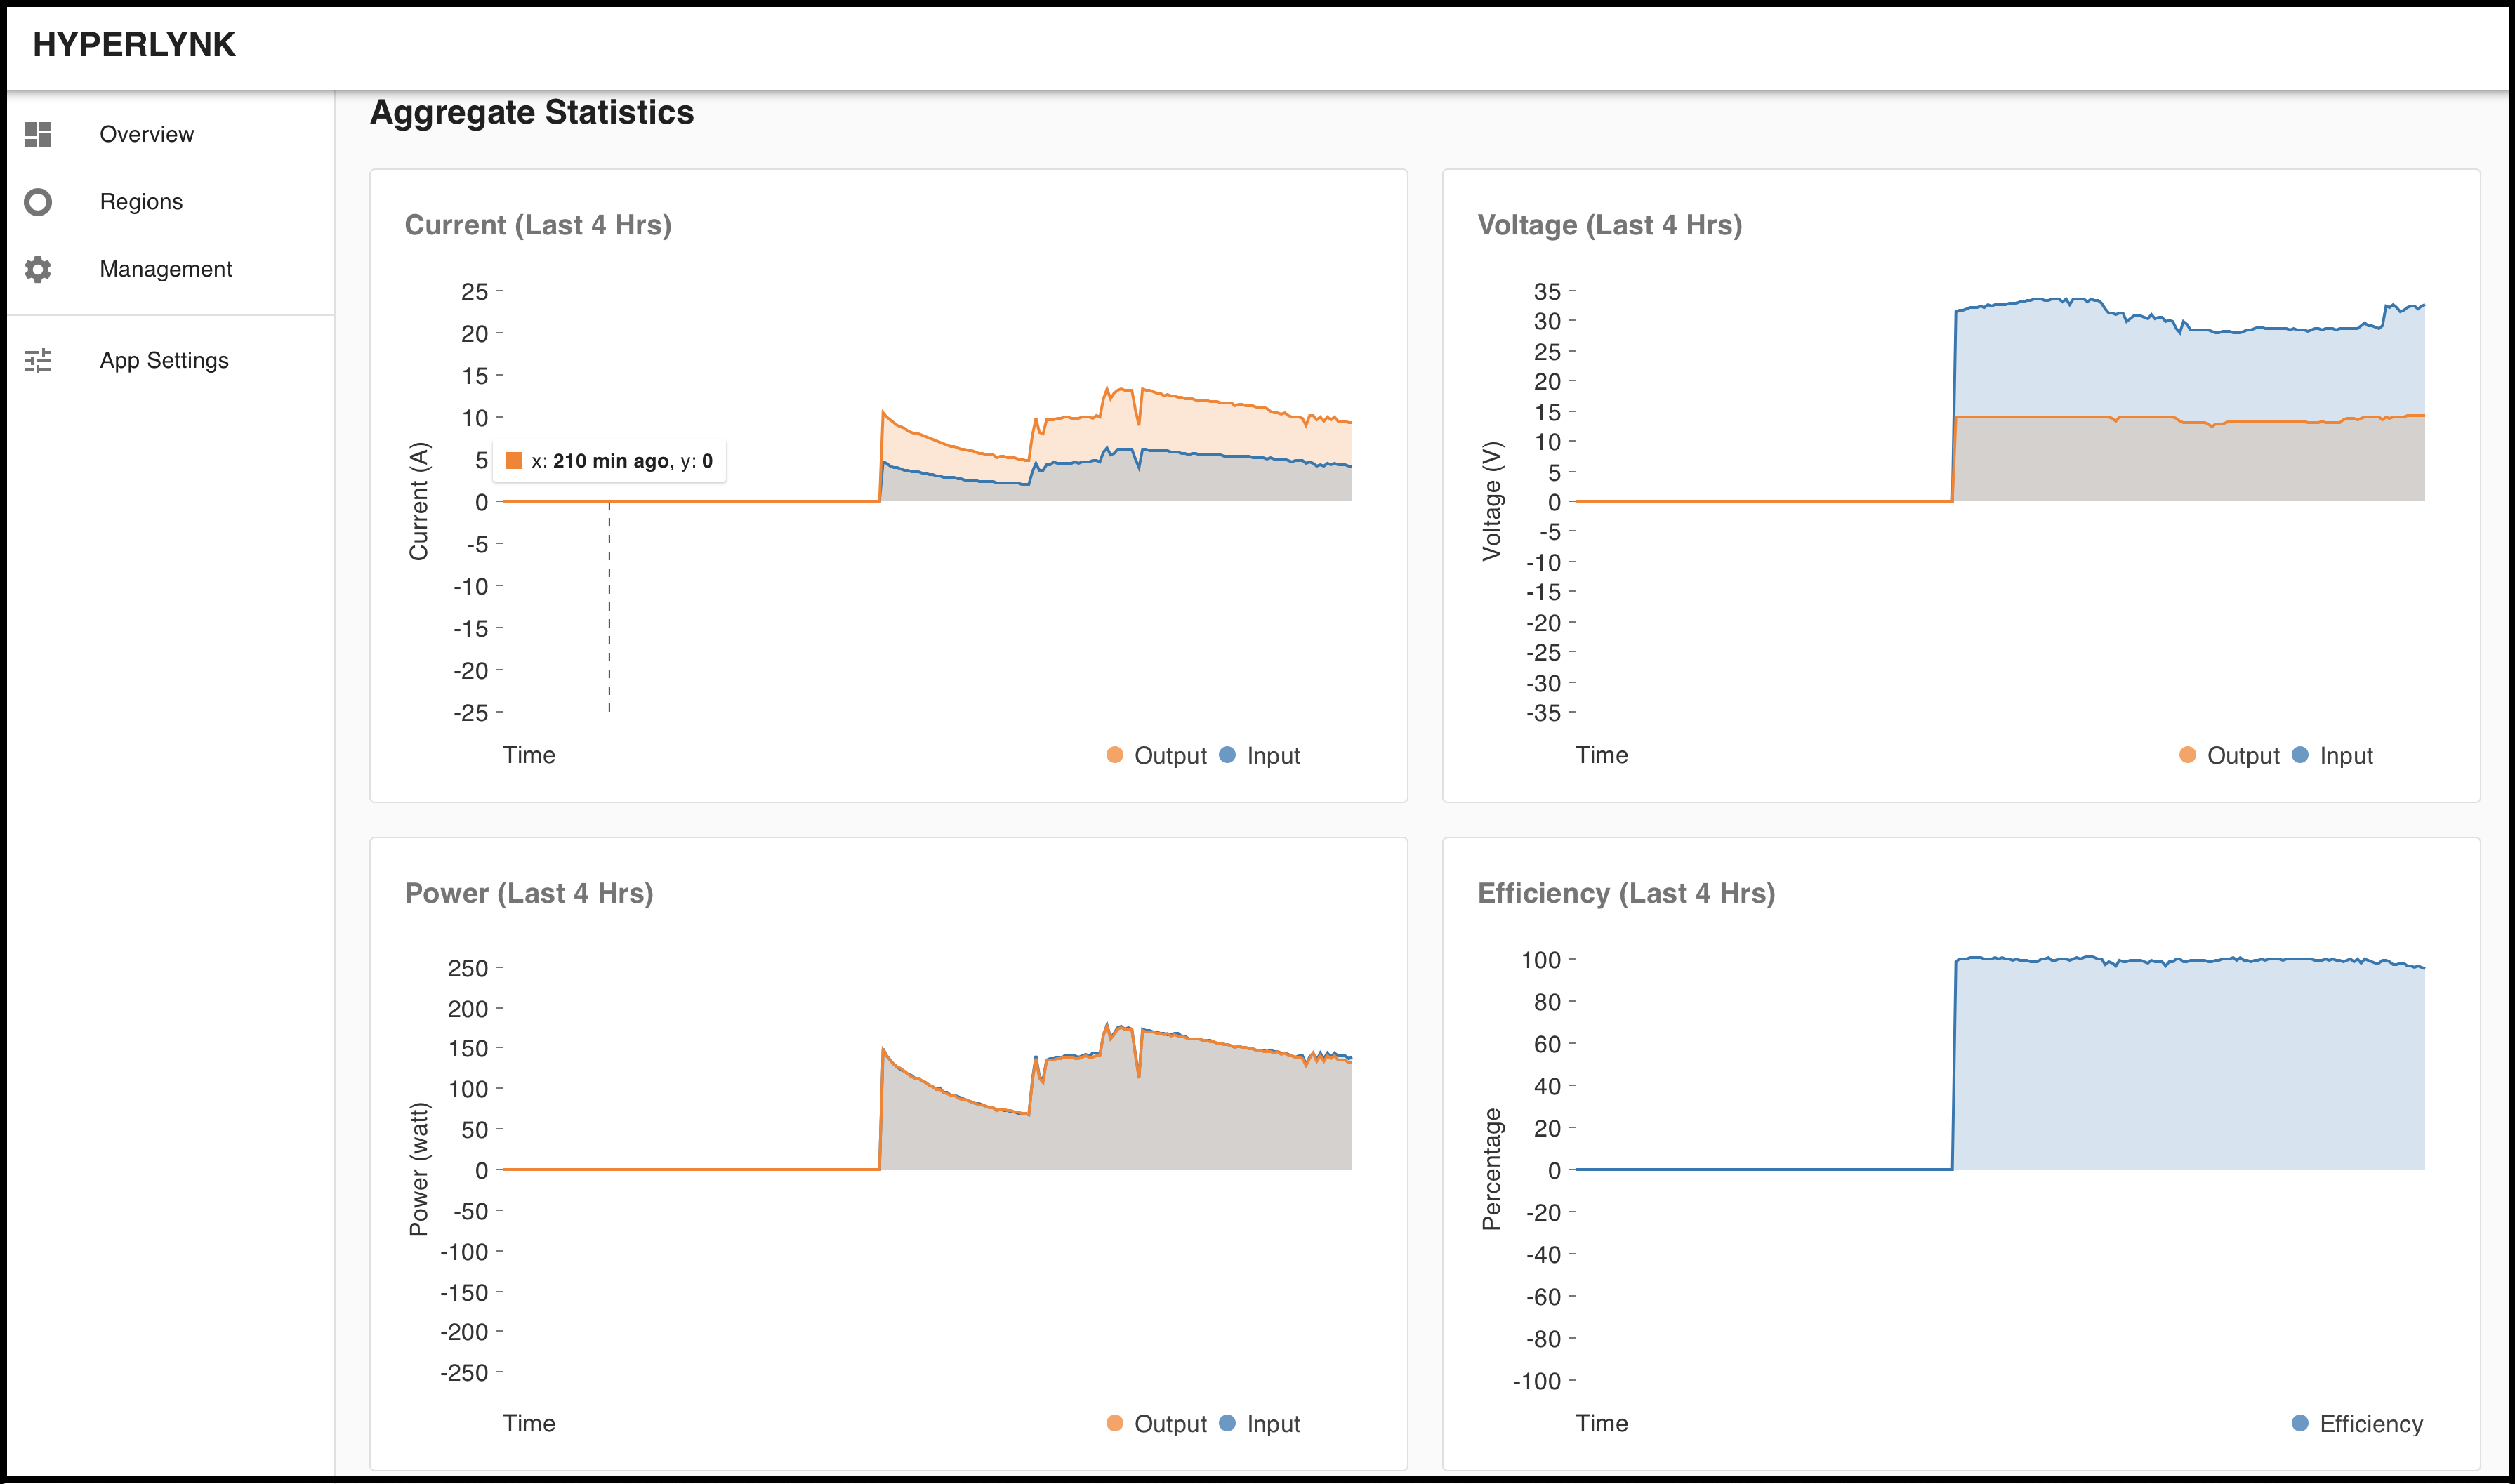
\includegraphics[width=\linewidth]{page2.png}
	\caption{The website showing the aggregate data.}
	\label{fig:page2}
\end{figure}

\begin{figure}[!ht]
	\centering
	\begin{subfigure}[b]{0.49\linewidth}
		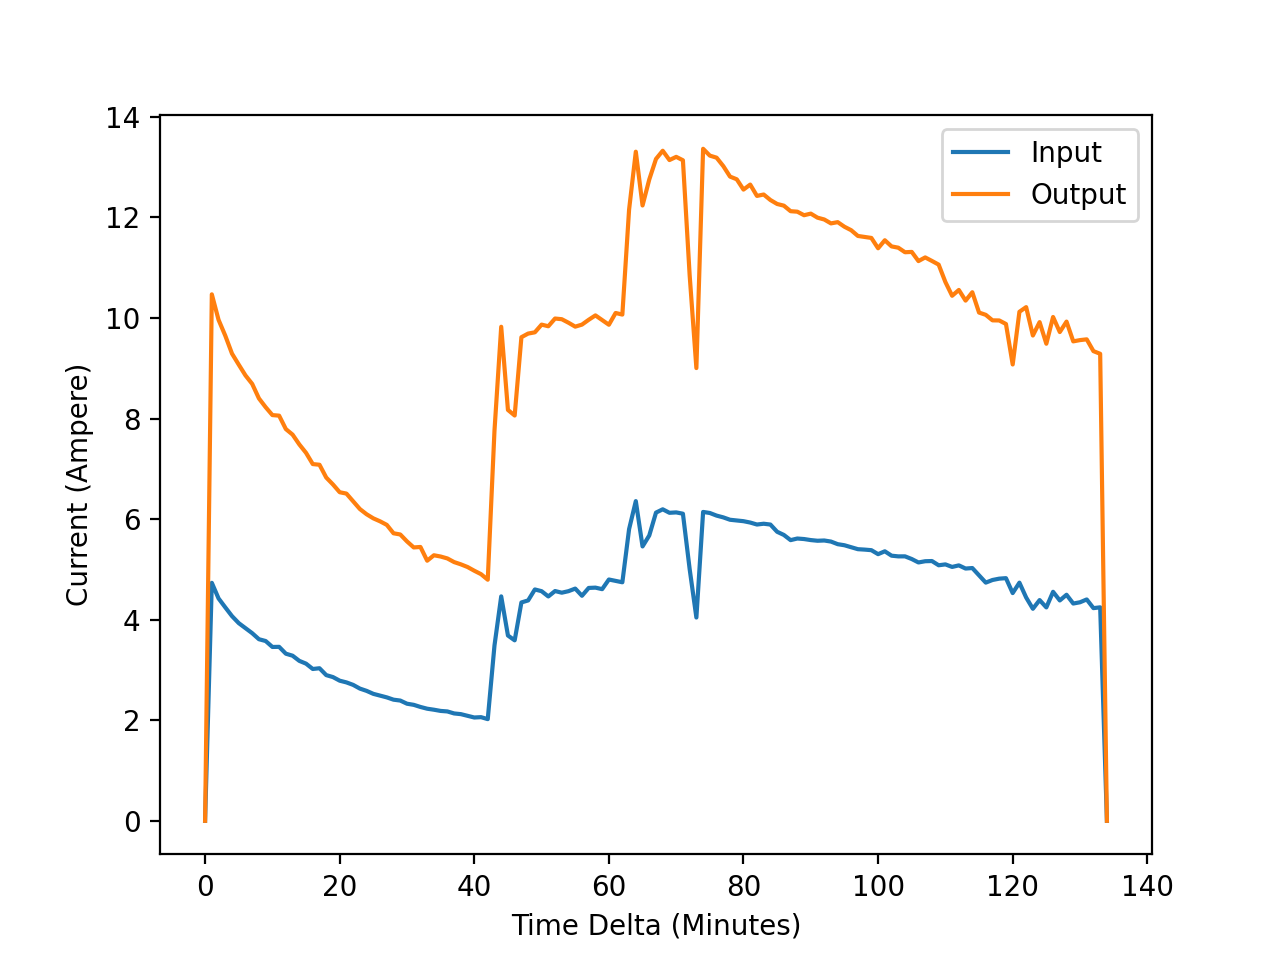
\includegraphics[width=\linewidth]{Current.png}
		\caption{Current}
	\end{subfigure}
	\begin{subfigure}[b]{0.49\linewidth}
		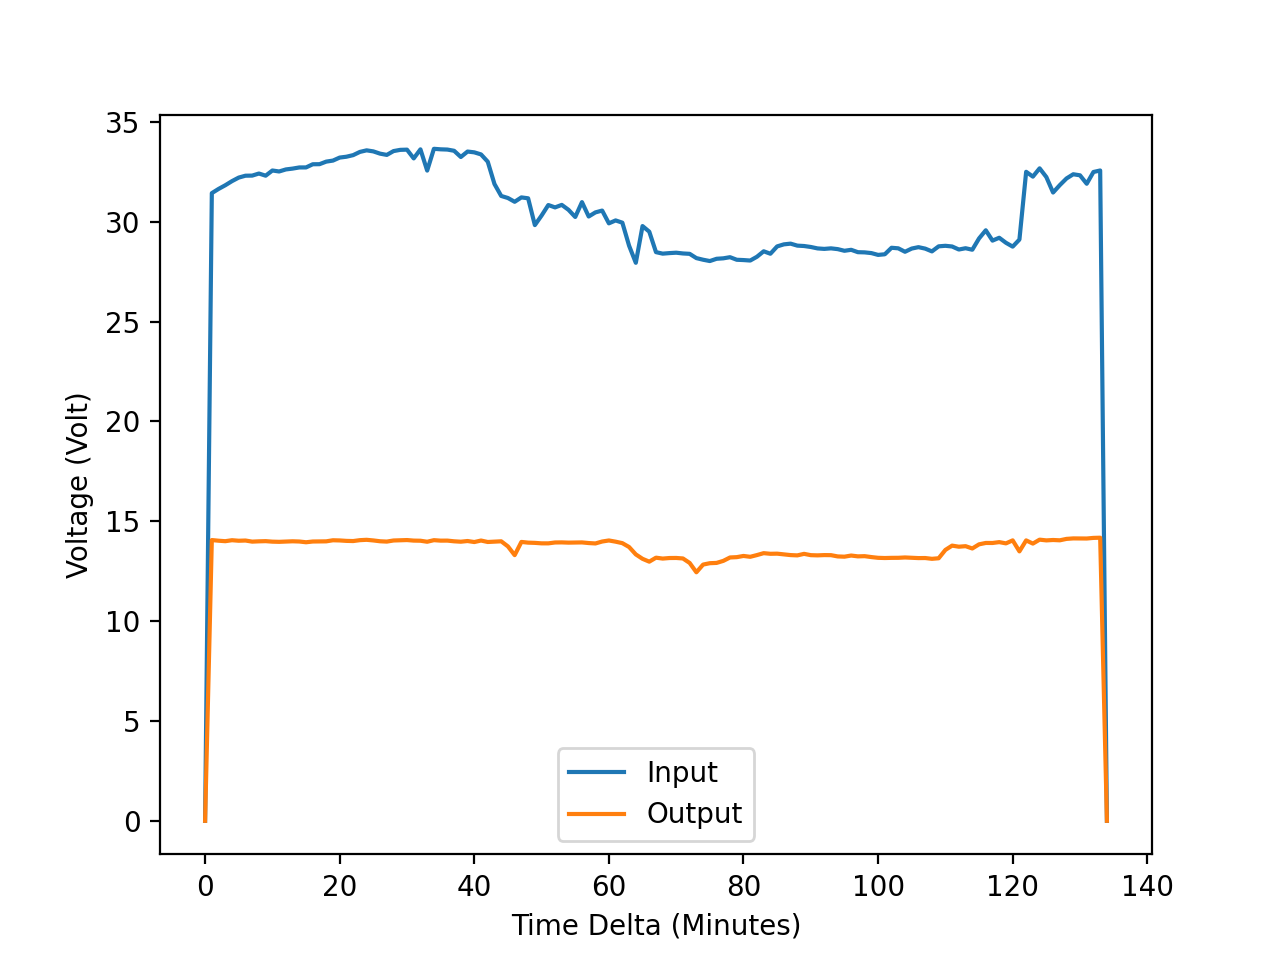
\includegraphics[width=\linewidth]{Voltage.png}
		\caption{Voltage}
	\end{subfigure}
	\begin{subfigure}[b]{0.49\linewidth}
		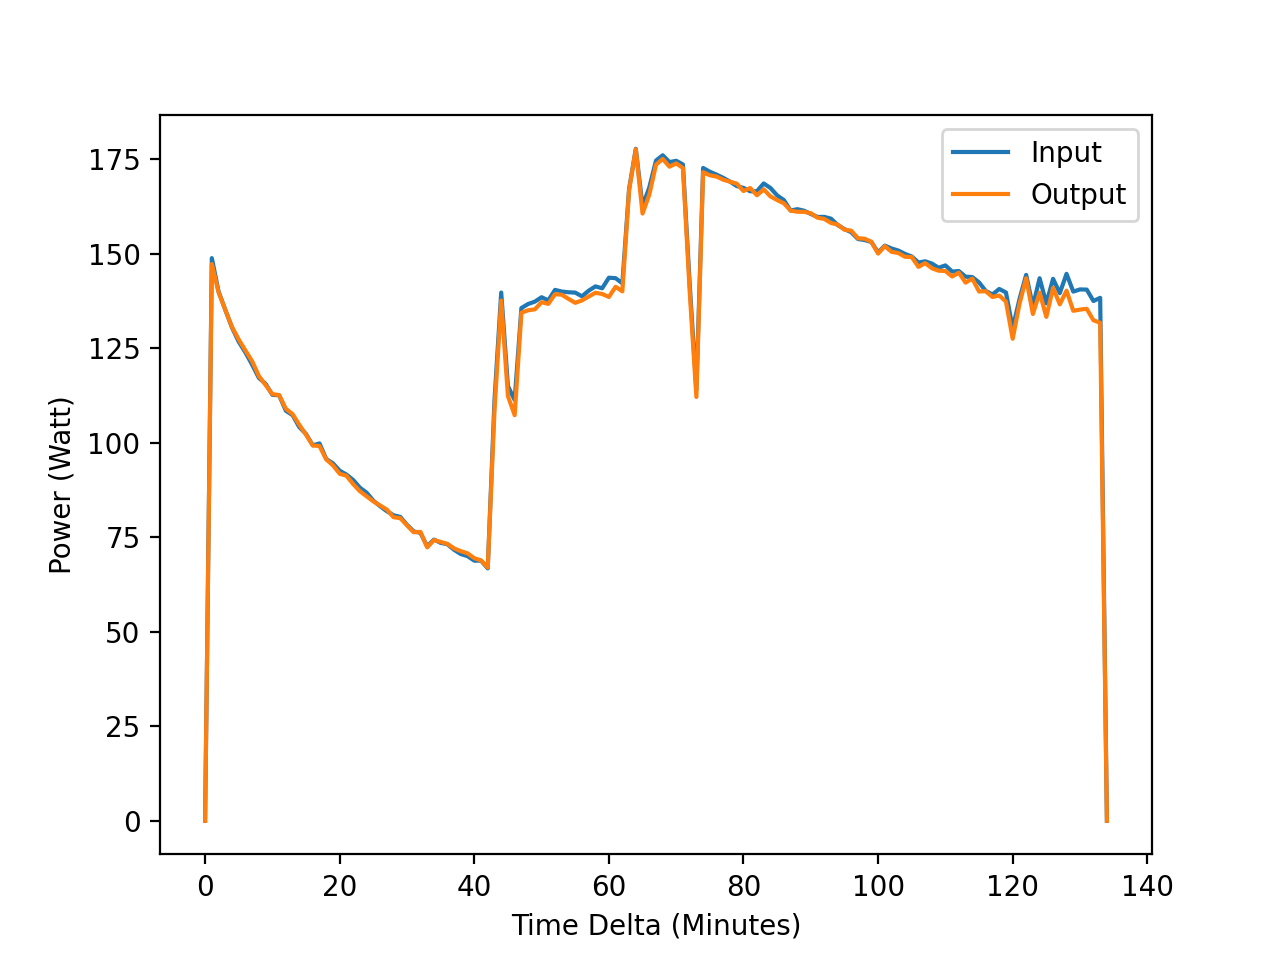
\includegraphics[width=\linewidth]{Power.png}
		\caption{Power}
	\end{subfigure}
	\begin{subfigure}[b]{0.49\linewidth}
		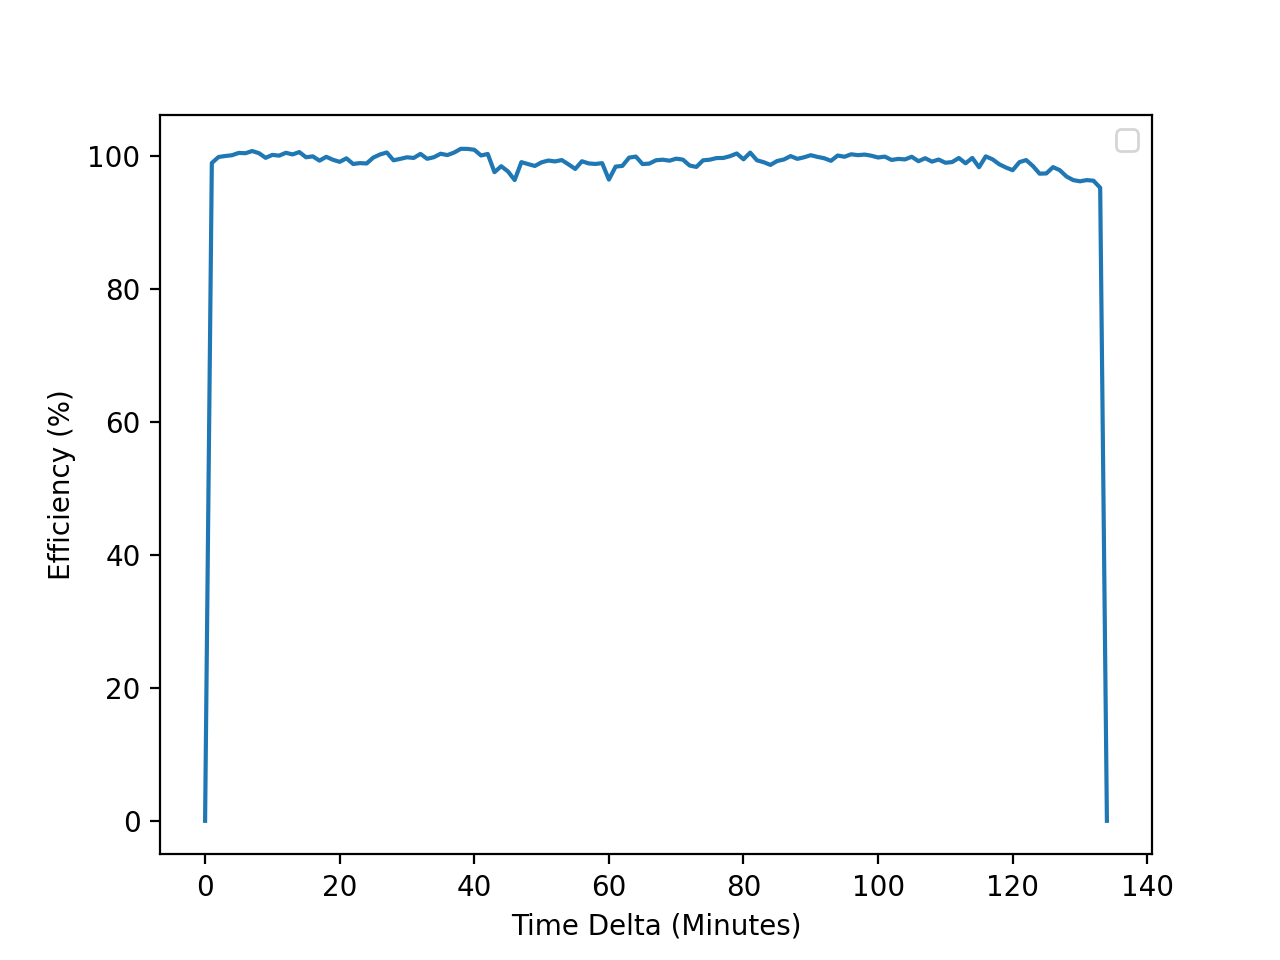
\includegraphics[width=\linewidth]{Efficiency.png}
		\caption{Efficiency}
	\end{subfigure}
	\caption{The captured data over a period of 2 hours.}
	\label{fig:captured}
\end{figure}

In the figure \ref{fig:page3}, the real-time statistics section shows the data that are being recorded in real-time and showing a maximum period of one minute before it is cleared and aggregated into the aggregate statistics. From the statistics, the device is working normally and generating power steadily for the last minute. 

\begin{figure}[!ht]
	\centering
	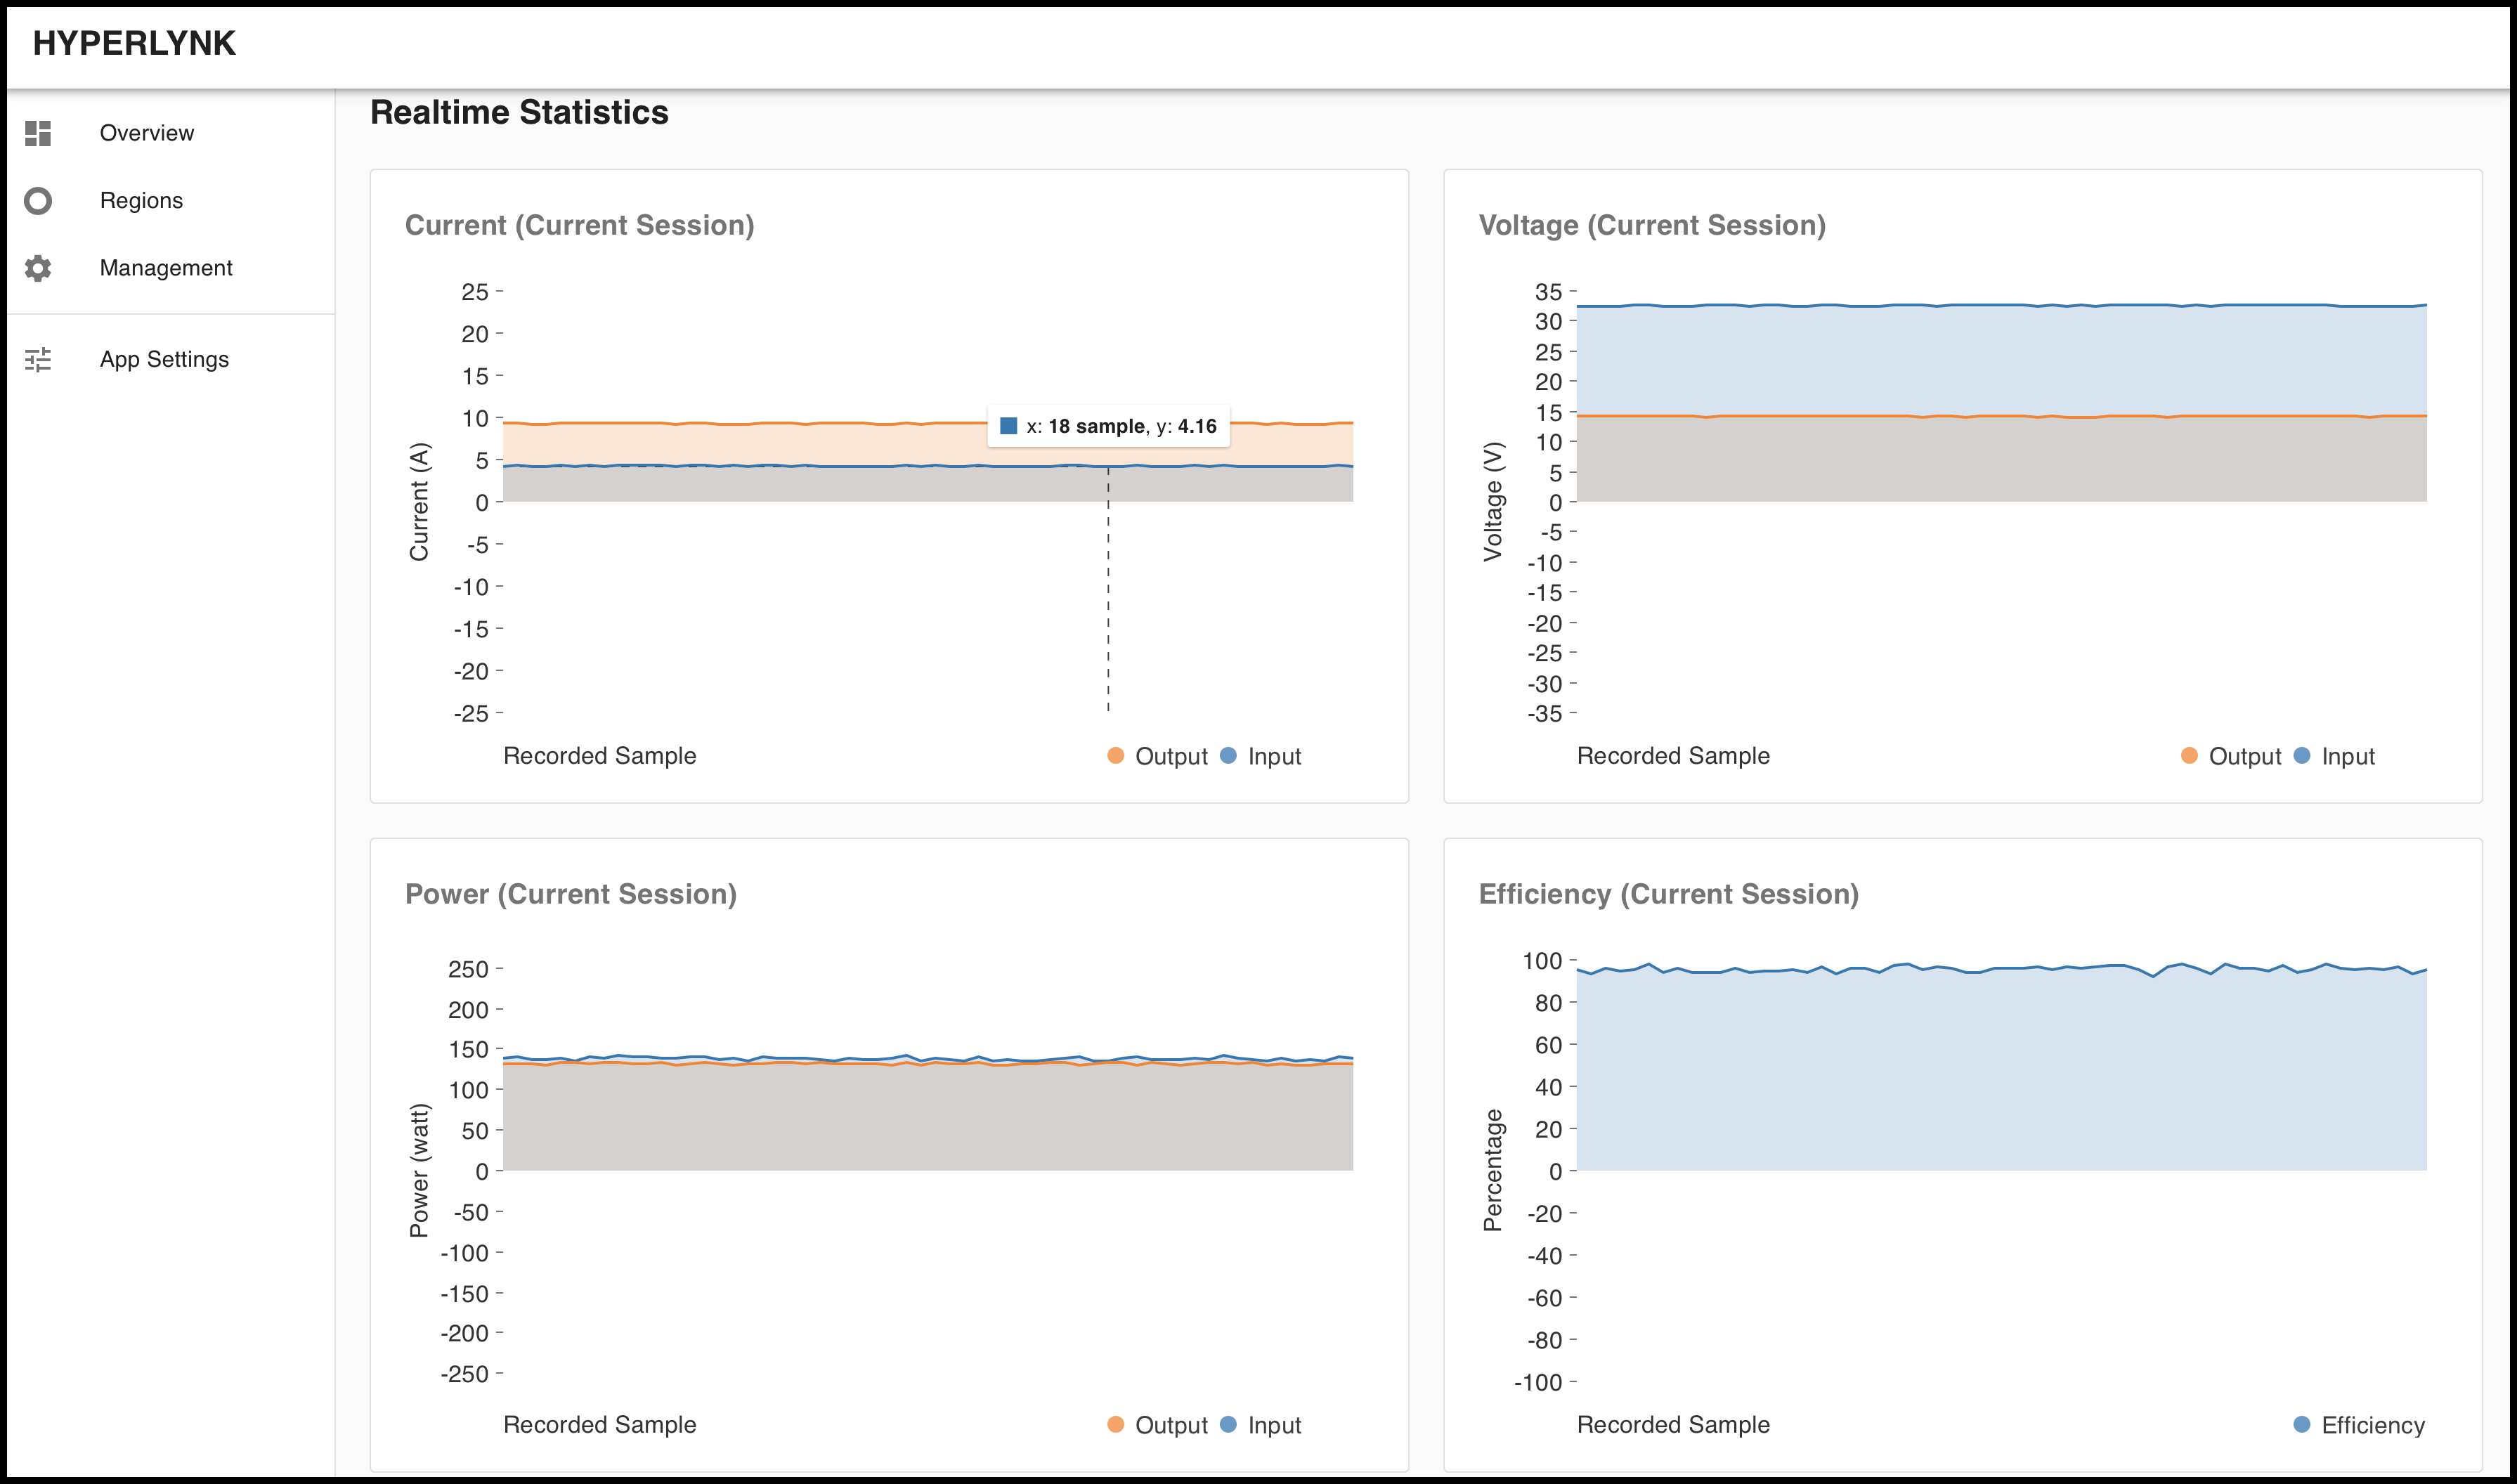
\includegraphics[width=\linewidth]{page3.png}
	\caption{The website showing the real-time data.}
	\label{fig:page3}
\end{figure}


Once the experiment is terminated properly, that means the device is being shutdown by using the commands provided on the webiste as shown in the figure \ref{fig:page4}. The status of the device is updated, as shown in the figure \ref{fig:offline}. 

\begin{figure}[!ht]
	\centering
	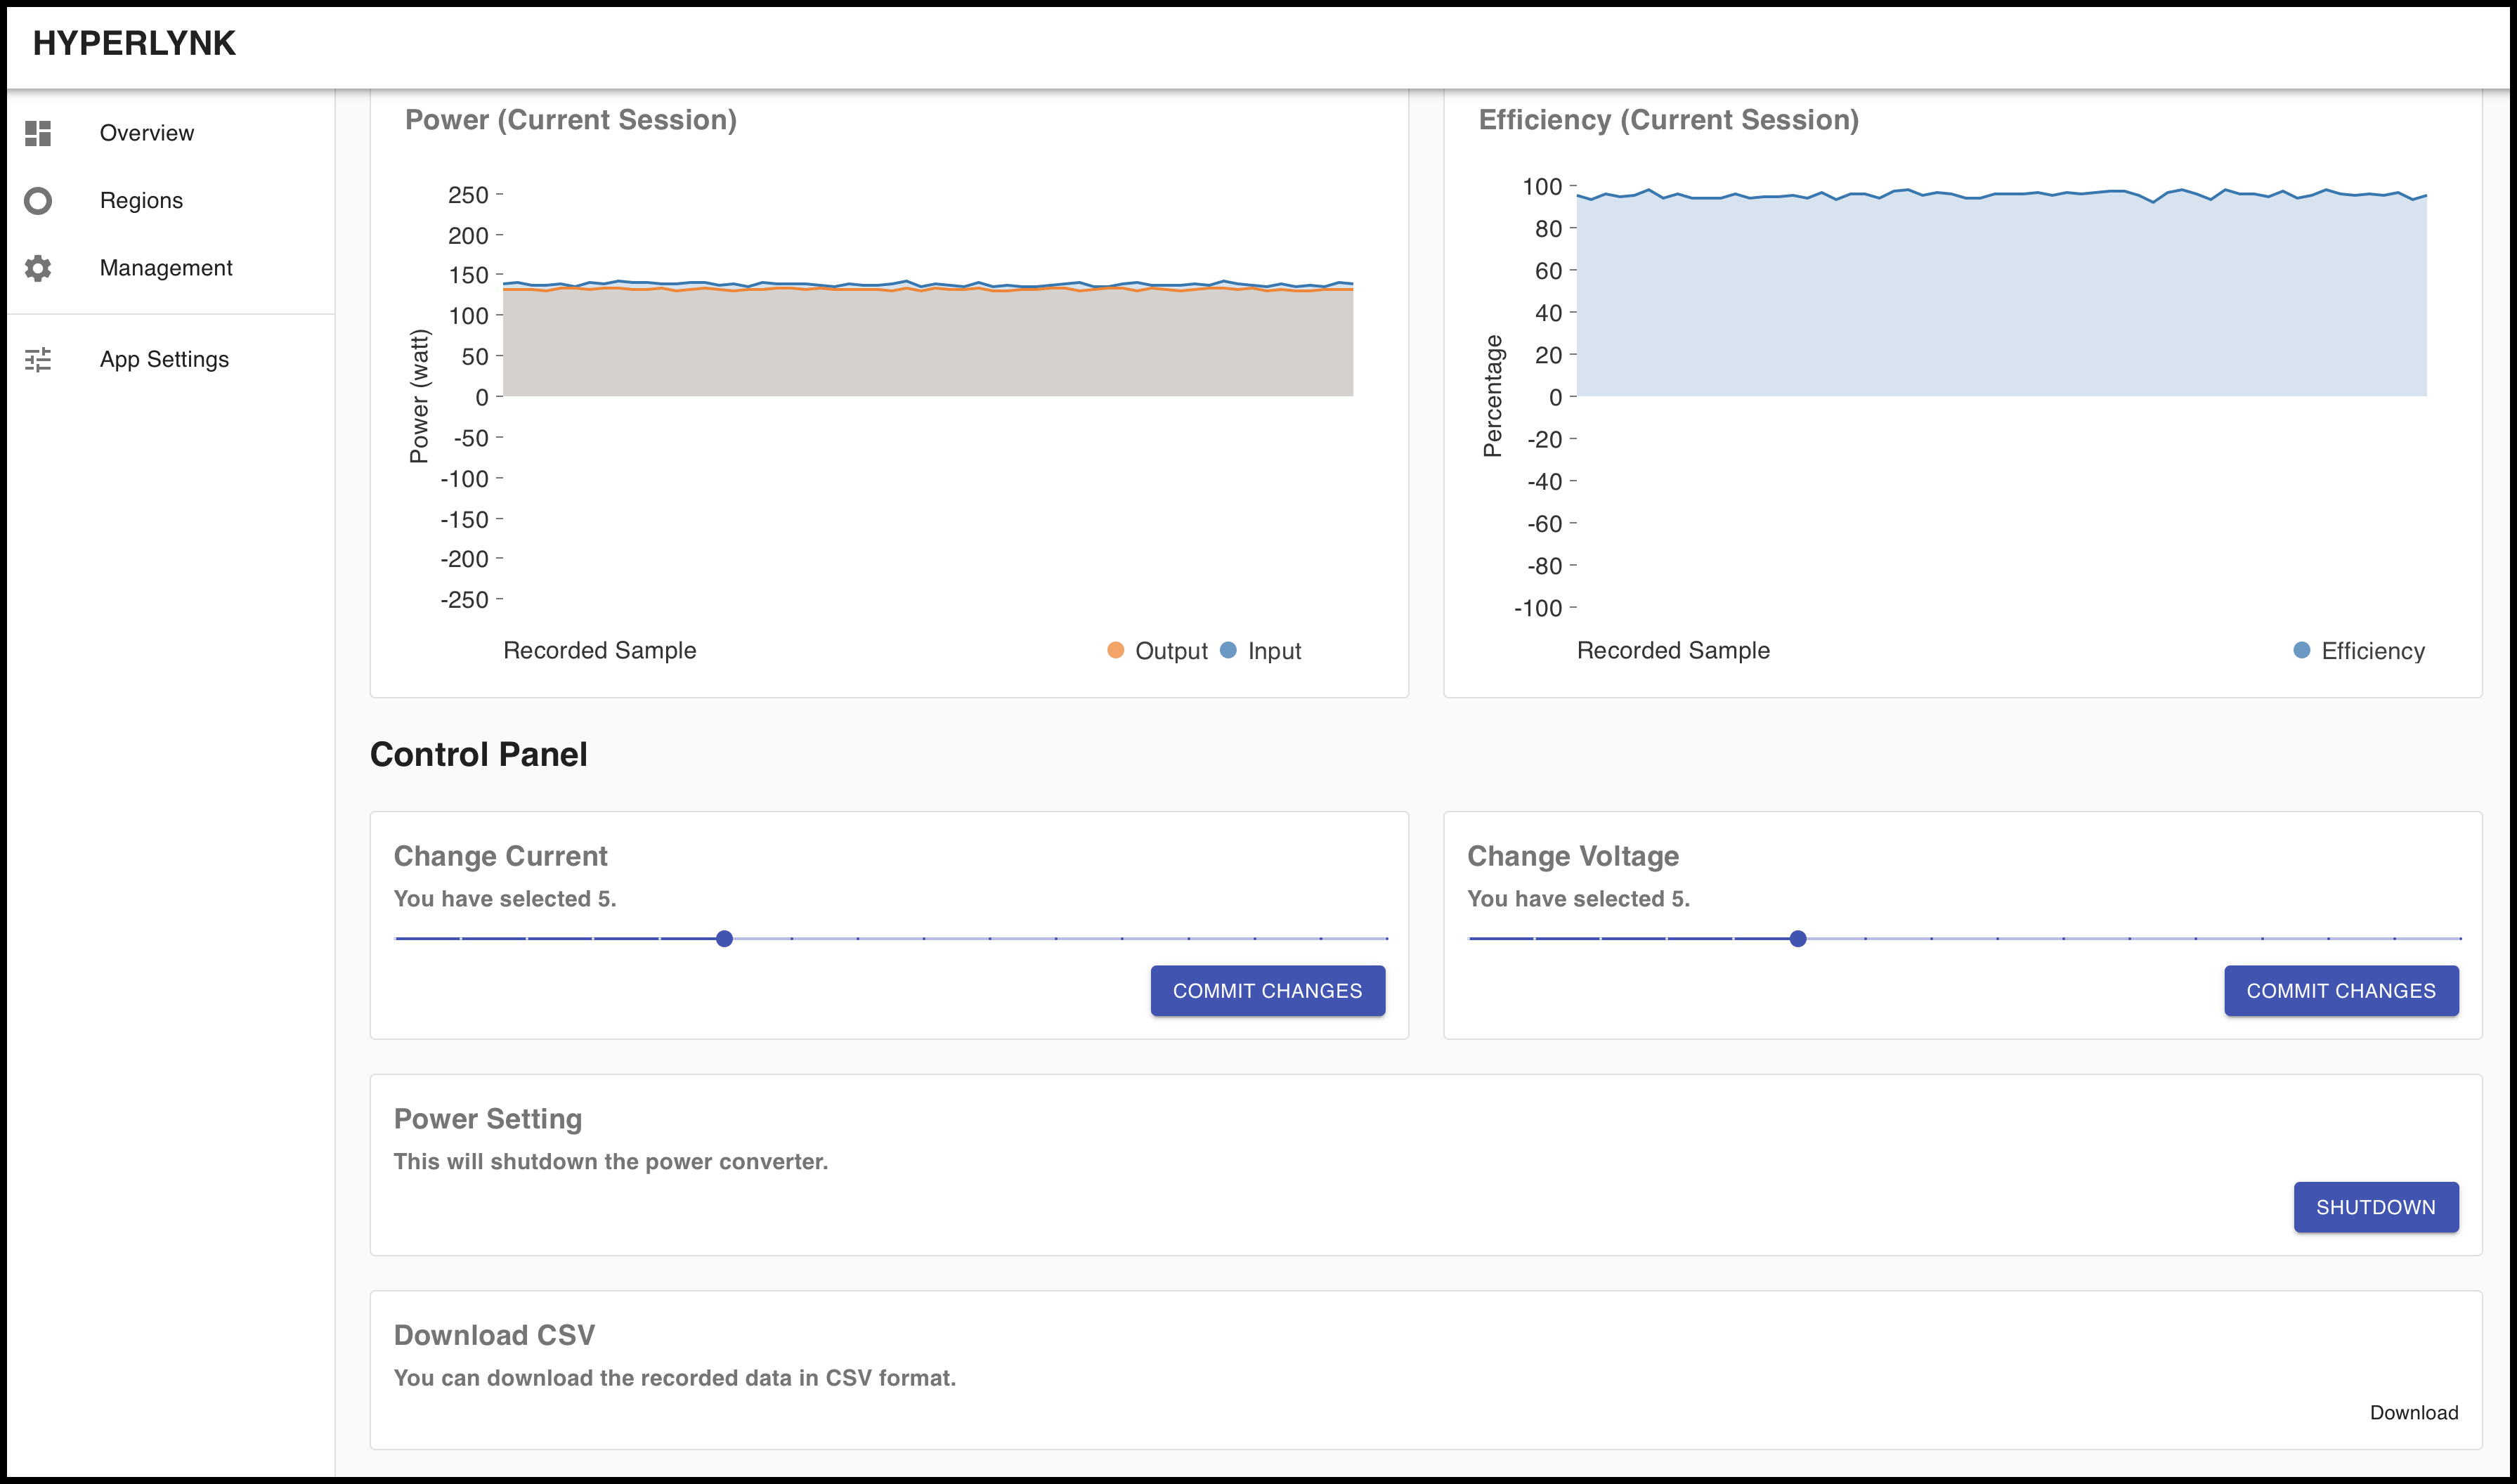
\includegraphics[width=\linewidth]{page4.png}
	\caption{The website's control panel.}
	\label{fig:page4}
\end{figure}

\begin{figure}[!ht]
	\centering
	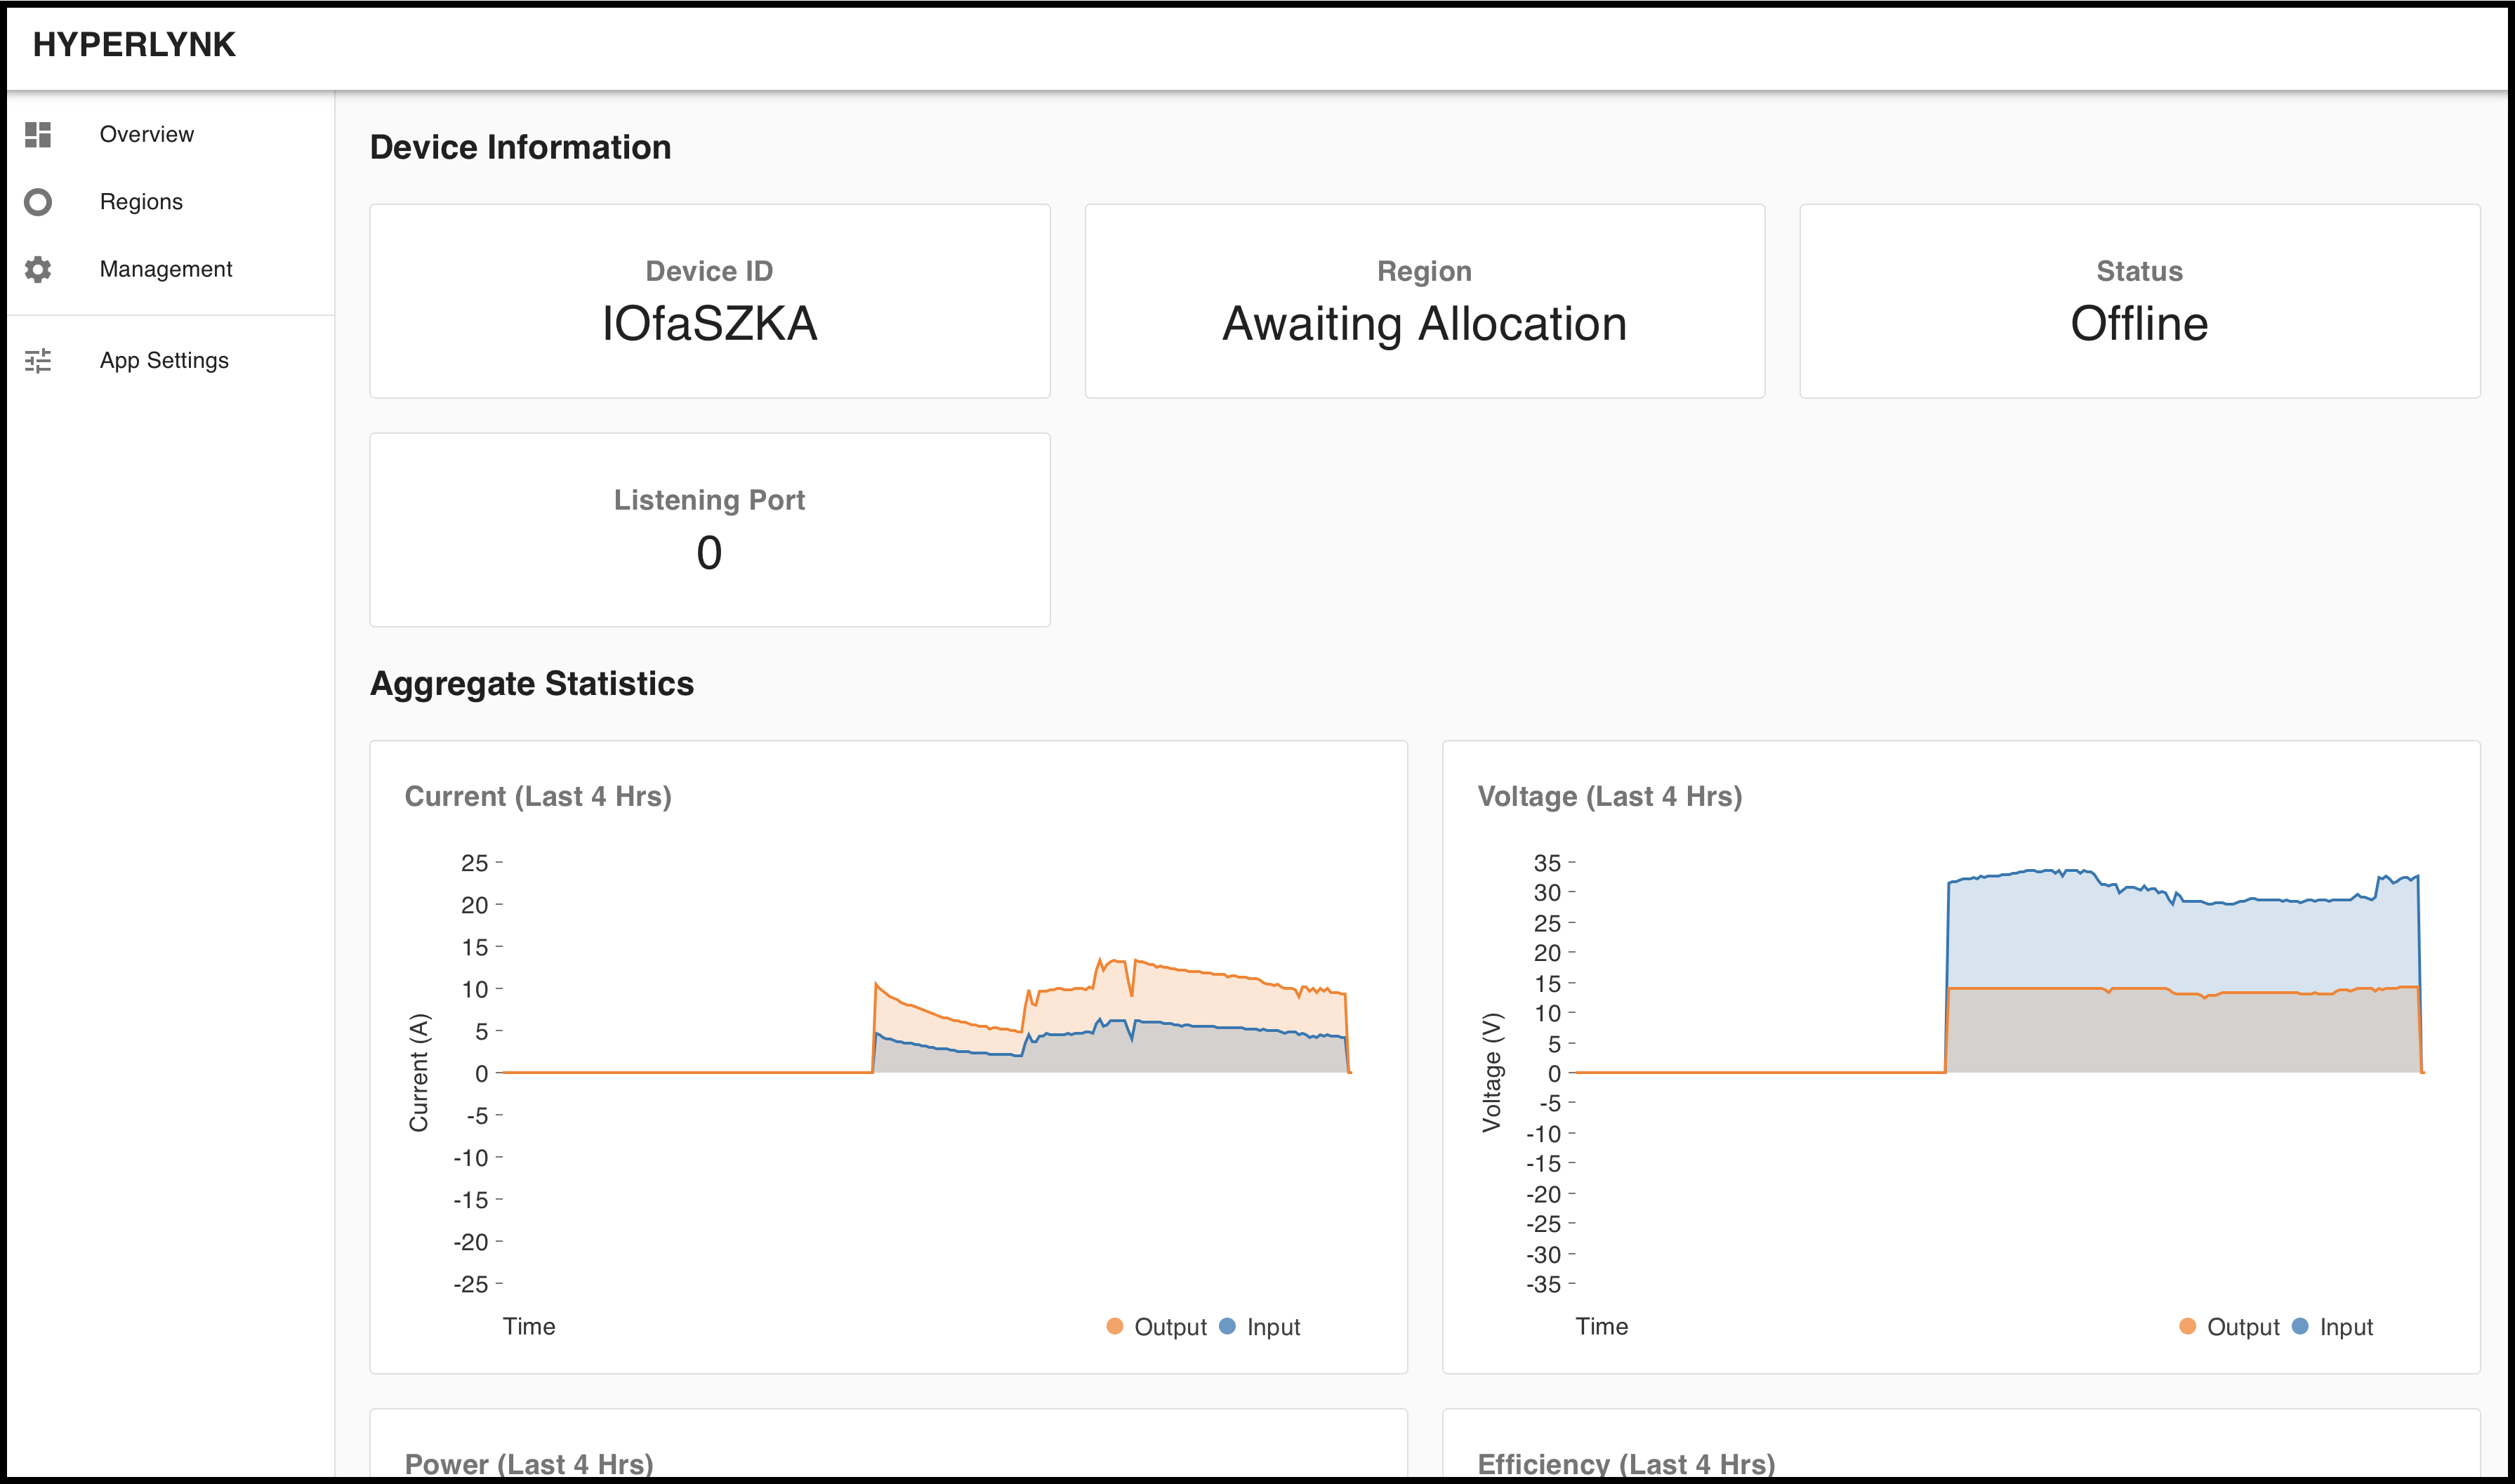
\includegraphics[width=\linewidth]{offline.png}
	\caption{The website shows the device is offline.}
	\label{fig:offline}
\end{figure}


Another experiment is conducted on a different day, where the testing aims to verify the accuracy of the data read by the sensor. We realised the data was inaccurate and turned off the power of the microcontroller directly without commanding it on the website. The website later detected the experimental device had been timed out and marked it as device failure. This is shown in the figure \ref{fig:failure}.


\begin{figure}[!ht]
	\centering
	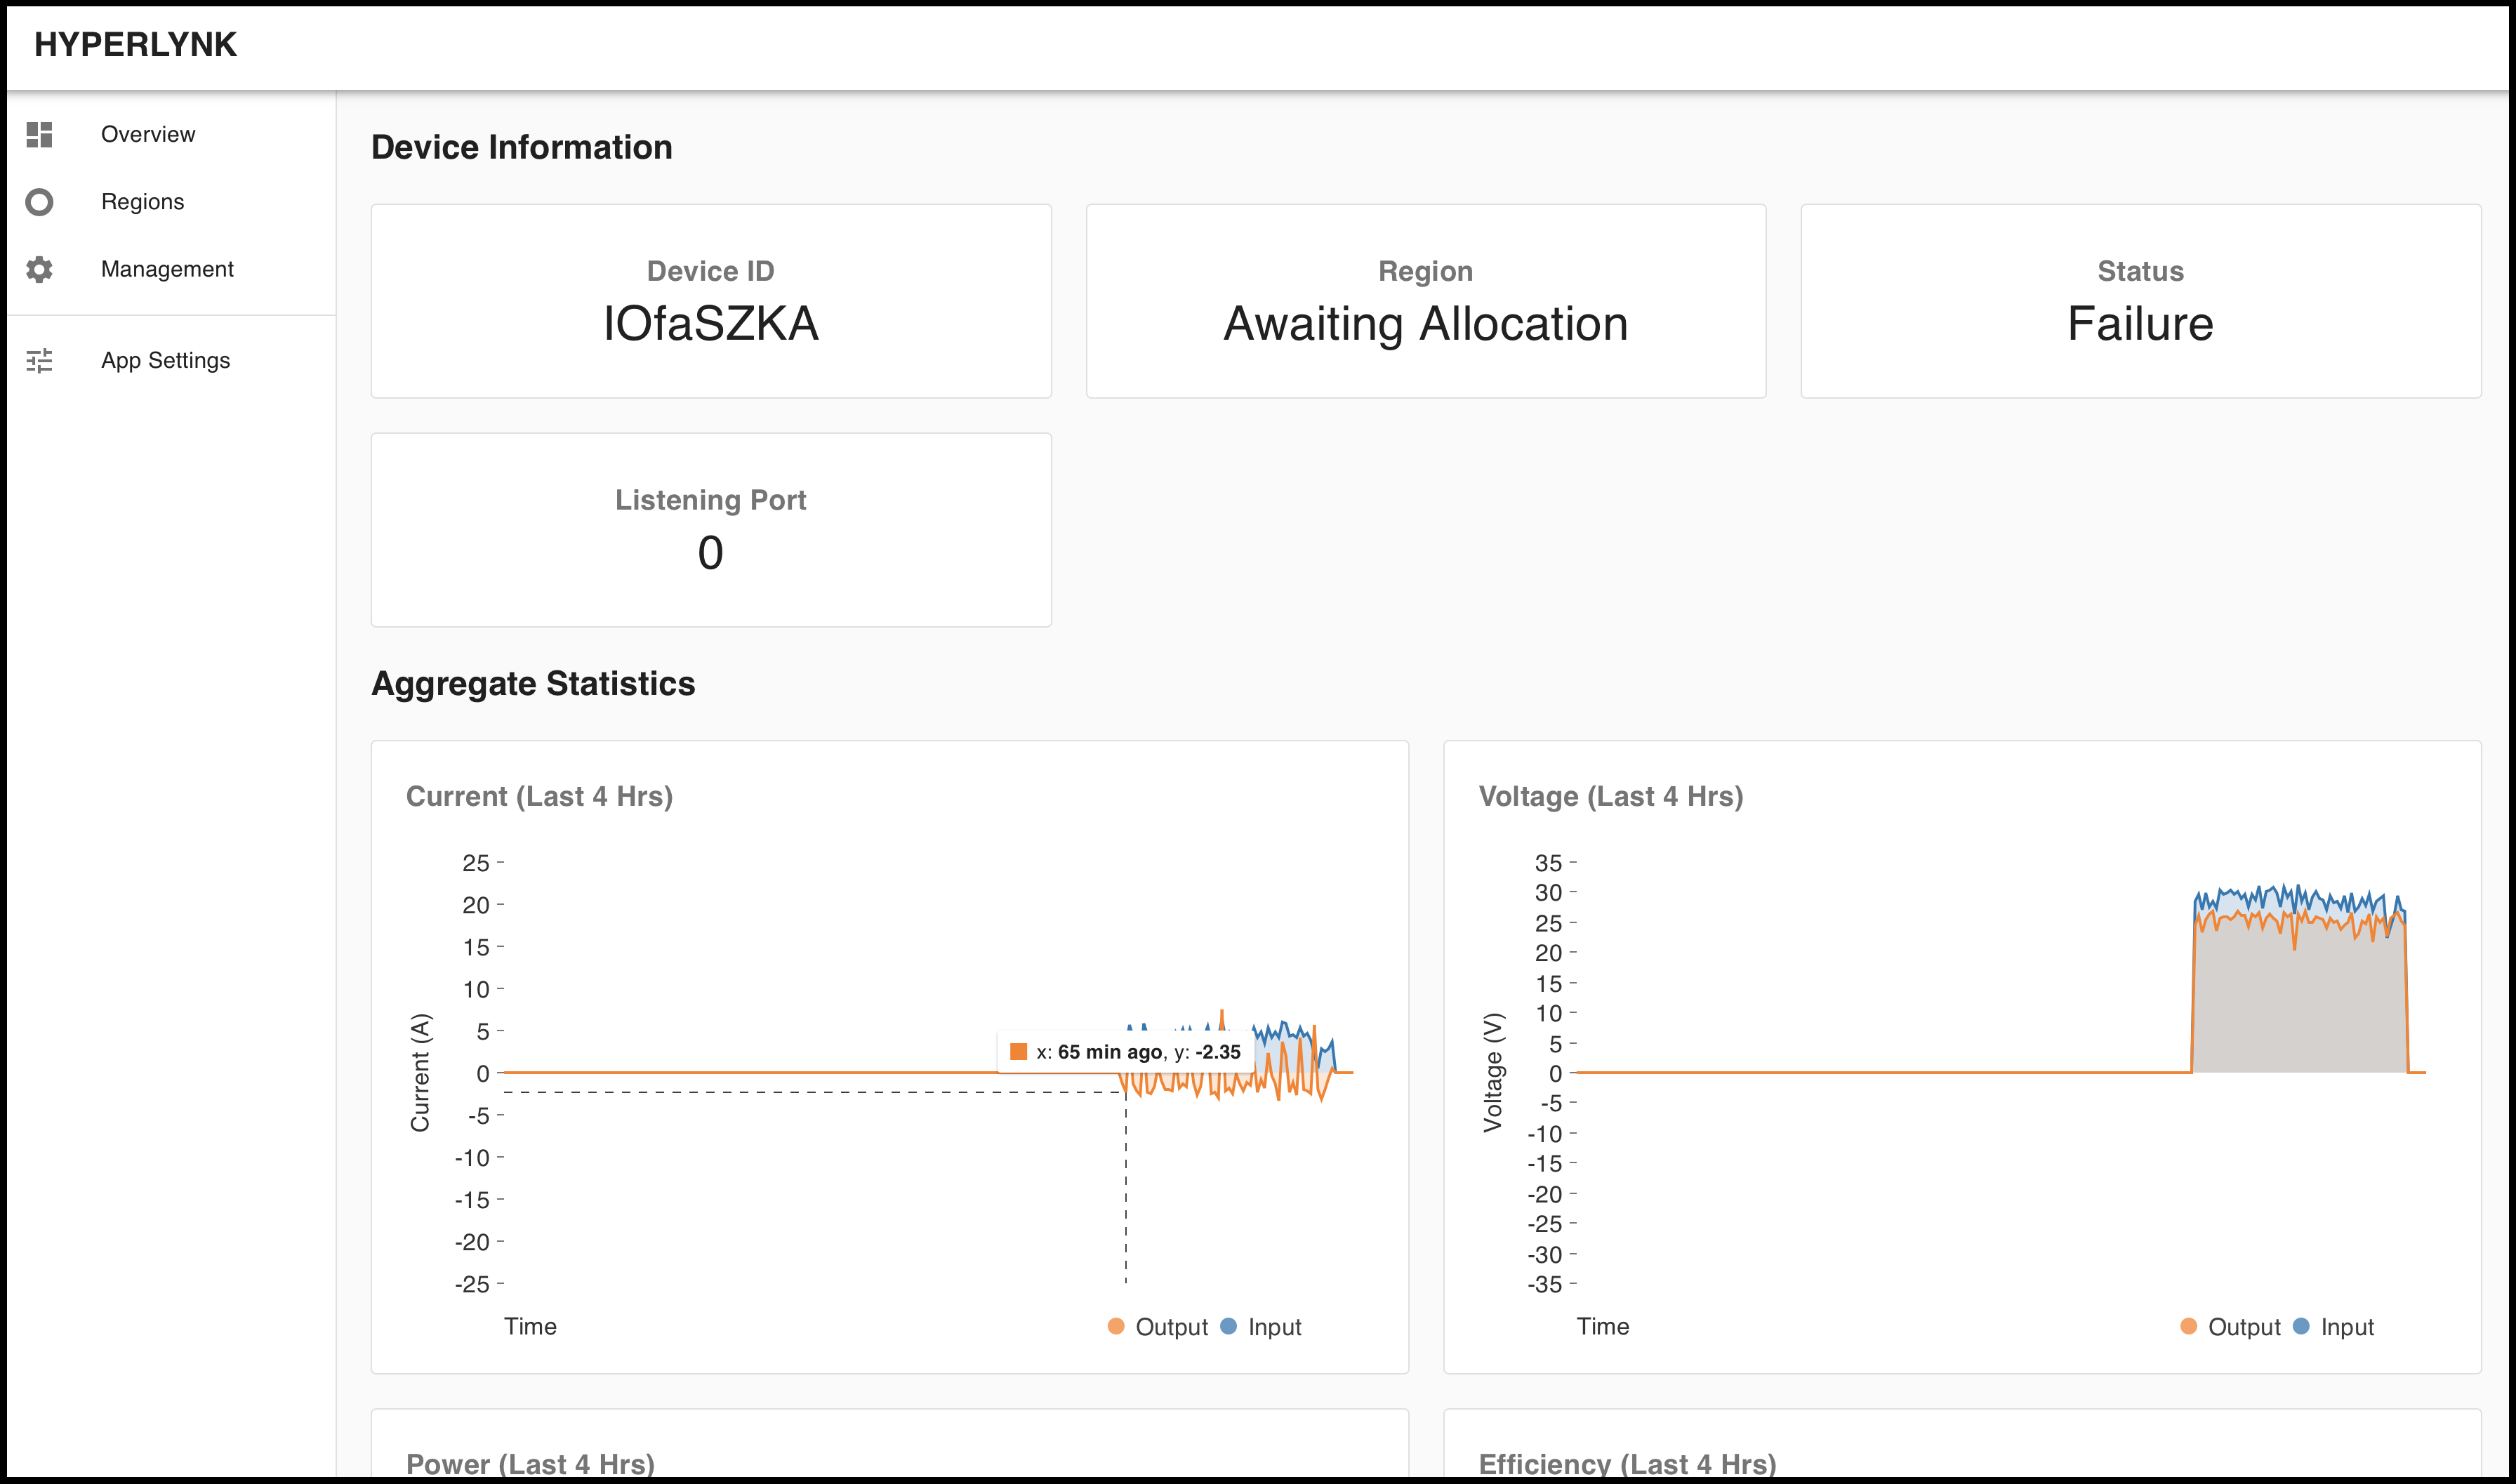
\includegraphics[width=\linewidth]{failure.png}
	\caption{The website shows the device has failed.}
	\label{fig:failure}
\end{figure}

\section{Conclusion}

During the real-world testing, the proposed system has shown it is capable of:

\begin{itemize}
	\item Storing sensing data.
	\item Showing sensing data.
	\item Receiving real-time data update.
	\item Controlling device behaviours.
\end{itemize}

Unfortunatly, device controlling capabilities are limited to shutting down the device only. This is due to the controlling system is depending on the work of another research student who is responsible for developing a custom converter and charger to replace the commercial product that we are using, and the comercial product does not allow us to control its behaviours. 

\end{document}